\documentclass[11pt,a4paper]{article}
\usepackage[UTF8]{ctex}
\usepackage[margin=2.3cm]{geometry}
\usepackage{graphicx}
\usepackage{booktabs}
\usepackage{longtable}
\usepackage{array}
\usepackage{amsmath}
\usepackage{amssymb}
\usepackage{float}
\usepackage{caption}
\usepackage{xcolor}
\usepackage{titlesec}
\usepackage{hhline}
\usepackage[hidelinks]{hyperref}

\graphicspath{{report_assets/}}

\titleformat{\section}{\large\bfseries}{\thesection}{0.8em}{}
\titleformat{\subsection}{\normalsize\bfseries}{\thesubsection}{0.8em}{}
\titlespacing*{\section}{0pt}{1.2ex}{0.6ex}
\titlespacing*{\subsection}{0pt}{0.9ex}{0.4ex}

\captionsetup{font=small,labelfont=bf}
\setlength{\parskip}{0.3em}
\newcommand{\rng}[2]{#1--#2}

\begin{document}

\begin{center}
{\LARGE\bfseries 基于真实数据与机器学习的高级选择权定价模型}\\[0.25em]
{\Large 8 周量化研究实习结项报告}\\[0.3em]
{\large Advanced Chooser Option Pricing Model with Real-World Data \& Machine Learning}\\[0.4em]
{\small 部门：Quantitative Research \& Trading \quad\textbar\quad 时长：8 周 \quad\textbar\quad 2026 年 8 月 26 日}\\[0.4em]
{\small \textbf{关键词：}选择权期权；Black--Scholes；波动率预测；机器学习；XGBoost；SHAP；Streamlit；双轨定价}
\end{center}

\begin{center}
\fbox{\parbox{0.92\linewidth}{\textbf{摘要：}本报告系统总结 8 周量化研究实习的完整工作。项目以 JPMorgan 选择权（Chooser Option）定价为主线，从真实市场数据出发，依次完成了数据采集与特征工程、BSM 模型复现与基线评估、机器学习双轨架构设计与训练调优、高级敏感性分析，并最终交付一套可部署的双轨定价工具。核心成果包括：调优后的 GBDT-anchored 波动率模型首次超越 persistence 强基线（MAE 7.16\% $<$ 7.32\%）；以市场隐含波动率为目标的 VIX-proxy 模型将合成测试集 Chooser 定价 MAE 从 \$1.52 降至 \$1.17（改善 23\%）；调优后的 XGBoost 在实盘快照上同时满足全部三项目标（实盘 MAE \$0.79、ATM IV 溢价 0.76\%、OTM 看跌偏差 $-29.5\%$）。情感/VIX 新特征被证明是价格的第一驱动因素。最终工具集成 BSM 与最优 ML 模型的双轨定价、误差条与完整可视化仪表板，形成从研究到落地的完整闭环。报告按周详细记录每一阶段的任务、方法、结果与交付物，汇总核心发现、交付清单与个人收获，并对局限性与未来方向进行了展望。}}
\end{center}

\section{项目概述与背景}

选择权期权（Chooser Option）赋予持有人在未来选择日 $t_1$ 决定该期权是欧式看涨还是欧式看跌的权利，并设定统一行权价 $K$ 与最终到期 $T_2$。作为结构化产品设计与风险管理的核心工具，它是连接学术模型（Black--Scholes）与行业实践的理想载体：一方面，选择权把方向选择权定价这一经典问题凝练为可解析求解的封闭式；另一方面，其价格对波动率的高度敏感使其天然成为检验波动率建模精度的试金石。

从业务价值看，选择权期权是三类应用场景的基础构件。在\textbf{结构化产品}中，它为具有明确方向性观点但对波动率或入场时机不确定的客户提供了灵活且成本高效的组合工具，投资者不必在期初就锁定看涨或看跌立场，而是把方向决策推迟到信息更充分的选择日；在\textbf{风险管理}中，它可以对冲非对称的、与市场环境相关的风险——例如财报发布后、FOMC 决策等事件驱动的波动，在事件结果公布前保留"两边下注"的权利；在\textbf{专有策略}中，选择权复杂的定价结构使其成为先进数值方法与模型校准的试验平台，其 Vega 敞口更是检验波动率预测模型精度的天然试纸。因此，能否对选择权期权进行准确、可解释、可部署的定价，直接关系到一个量化部门的定价能力与对冲效率。

本项目以"基于真实数据及机器学习的 Chooser 期权定价"为主题，在 8 周内完成五个层面的目标：其一，利用 2018--2024 年真实市场数据重新构建并验证基于 BSM 的选择权定价模型；其二，采集多维度实时/历史数据以丰富定价特征；其三，开发机器学习模型优化波动率预测与期权定价，以解决 BSM"恒定波动率"的根本局限；其四，将 ML 增强模型与传统 BSM 系统对比，量化性能提升；其五，交付一套数据驱动、可扩展、可部署的定价工具与投资洞察。

表 \ref{tab:timeline} 给出 8 周的任务与交付物总览。项目按"数据 $\to$ 模型 $\to$ 工具"三阶段推进，每周产出独立实验报告，最终汇成本结项报告。

\begin{table}[H]
\centering
\caption{8 周任务与交付物总览}
\label{tab:timeline}
\begin{tabular}{@{}cllp{0.42\linewidth}@{}}
\toprule
周次 & 核心模块 & 关键任务 & 交付物 \\
\midrule
1 & 数据源设计与采集 & API 配置、JPM/VIX/3M 国债采集 (2018--2024) & 数据规范、API 脚本、原始数据集 \\
2 & 预处理与特征工程 & 清洗、16+ 维特征、自动化 Pipeline & 结构化数据集、Pipeline 代码、特征文档 \\
3 & BSM 模型复现 & Rubinstein 解析公式、MC 验证、敏感性 & BSM 代码、验证 Notebook、参数配置 \\
4 & 基线评估 & MAE/RMSE、局限分析、基准建立 & 验证报告、性能基准、优化后 BSM 代码 \\
5 & ML 模型设计 & 双轨架构、时序分割、初始模型框架 & 架构文档、特征优化代码、初始 ML 框架 \\
6 & 训练调优比较 & 超参优化、测试集评估、SHAP/LIME & 训练模型 pkl、比较报告、SHAP 图 \\
7 & 高级分析工具 & SHAP$\times$Vega、极端场景、工具原型、实时数据 & 敏感性报告、Streamlit 原型、数据更新模块 \\
8 & 工具完善交付 & 双轨定价、误差条、完整仪表板、最终报告 & 可部署工具、最终报告、演示文稿与脚本 \\
\bottomrule
\end{tabular}
\end{table}

\section{总体架构与技术路线}

项目采用"学术模型（BSM）$\to$ 机器学习增强 $\to$ 工具化部署"的三阶段技术路线，并在整个过程中贯彻反前瞻偏差（look-ahead bias）工程纪律。

在模型层面，项目设计了\textbf{双轨架构}（第 5 周定型）：\textbf{方法一}（两阶段、可解释）由 ML 模型预测 BSM 唯一的未知输入——波动率 $\hat\sigma$——再代入第 3 周验证的 Rubinstein 公式定价；\textbf{方法二}（单阶段、数据驱动）由监督学习直接从"市场特征 + 合约参数"学习定价映射。两条路径共享同一套特征工程与时序分割管线，最终统一与 BSM($\sigma_{21d}$) 基线对比。

在数据层面，反前瞻保障贯穿六重环节：时序 70/15/15 分割且禁止 shuffle、train/val/test 边界各剔除 21 日（purge/embargo）、特征全部采用滚动/滞后后视窗口、目标与特征日期严格错开、Scaler 仅在训练集拟合、LSTM 窗口严格不超过锚点。这些措施由 38 项自动化测试逐条断言验证。反前瞻纪律的意义在于：金融时间序列与独立同分布样本不同，若任一环节使用了未来信息，模型的测试集表现将被系统性高估，无法反映真实部署时的预测能力。因此，项目将"可复现、无泄漏"作为与"预测精度"同等重要的工程目标，所有模型训练、调优与评估均在统一的分割框架下进行，保证跨周结论可比。

在方法学上，项目遵循"先诊断、再建模、后验证"的推进原则：第 4 周先以实证数据诊断 BSM 的失效模式（波动率时变、微笑、情绪缺口），第 5 周据此设计针对性更强的双轨架构，第 6 周再用严格的测试集评估量化改进。每一阶段的结论都作为下一阶段的设计输入，形成证据驱动的迭代闭环。

\section{分周工作内容与成果}

\subsection{第 1 周：数据源设计与初步采集}

本周完成数据需求设计、API 管线搭建与初始数据采集三项目标。数据需求覆盖金融市场价格（JPM OHLCV）、市场恐慌代理（VIX 指数）与宏观经济（3 个月国债收益率，作为无风险利率代理）三类，时间窗口为 2018-01--2024-12（7 年，覆盖 COVID 危机、高通胀与美联储加息周期）。数据需求文档明确定义了每类数据的字段、来源、频率与用途：JPM OHLCV 用于期权定价的基础资产，VIX 作为市场恐慌/波动率代理，3M 国债收益率作为无风险利率代理——三类数据共同构成后续所有模型输入的原始素材。

数据管线采用多源冗余设计：以 Yahoo Finance 直连 Chart API v8 为主源（因 yfinance 库被限流，改用浏览器模拟 Header + 指数退避重试），Alpha Vantage 与 FRED REST API 为备选。最终采集 JPM 日线 1760 行、VIX 1760 行、3 个月国债 1750 行，三源均无缺失值与重复行。多维度联合分析显示：JPM 与 3M 国债收益率正相关（0.475），与 VIX 负相关（$-0.355$），3M 与 VIX 负相关（$-0.384$）——金融危机期间 JPM 股价与 VIX 的负联动得到验证。图 \ref{fig:w1} 展示了三个时间序列的 7 年走势：2020 年 3 月 COVID 暴跌时 JPM 大幅下挫、VIX 飙升至 35 以上，2022 年加息周期中收益率显著上行。JPM 股价在 2018--2020 年区间于 \$79--\$137 区间运行，2021 年起随大盘上行，2024 年末收于 \$221；VIX 均值 19.87、范围 9.15--82.69，2020 年 3 月飙升至 80 以上（危机峰值）后回落；3M 国债收益率均值 2.43\%，2020 年跌至 0 附近、2022--2023 年加息周期升至 5.63\%。三个序列的联动特征清晰可辨：风险事件期 JPM 下跌与 VIX 上行同步，而收益率在宽松期走低、紧缩期走高，为后续特征工程中的跨资产联动与利率动量设计提供了直接依据。

数据采集中遇到并解决了三类实际问题。其一，\textbf{Yahoo Finance 限流}：yfinance 库请求被 Yahoo 限流（YFRateLimitError），改为直连 Yahoo Chart API v8，通过浏览器模拟 Header 与指数退避重试规避限流；其二，\textbf{Alpha Vantage 付费限制}：其日线调整端点 TIME\_SERIES\_DAILY\_ADJUSTED 为 Premium 端点，免费版仅返回最近 100 天，不满足 7 年窗口，因此降级为备选源；其三，\textbf{数据长度不一致}：JPM（1760 行）与 3M 国债（1750 行）交易日数不同，采用按日期 inner join 对齐，保证相关性分析只基于双方都有的日期。数据质量评估确认三个源均无缺失值与重复行，为后续特征工程提供了干净可靠的基础。

\begin{figure}[H]
\centering
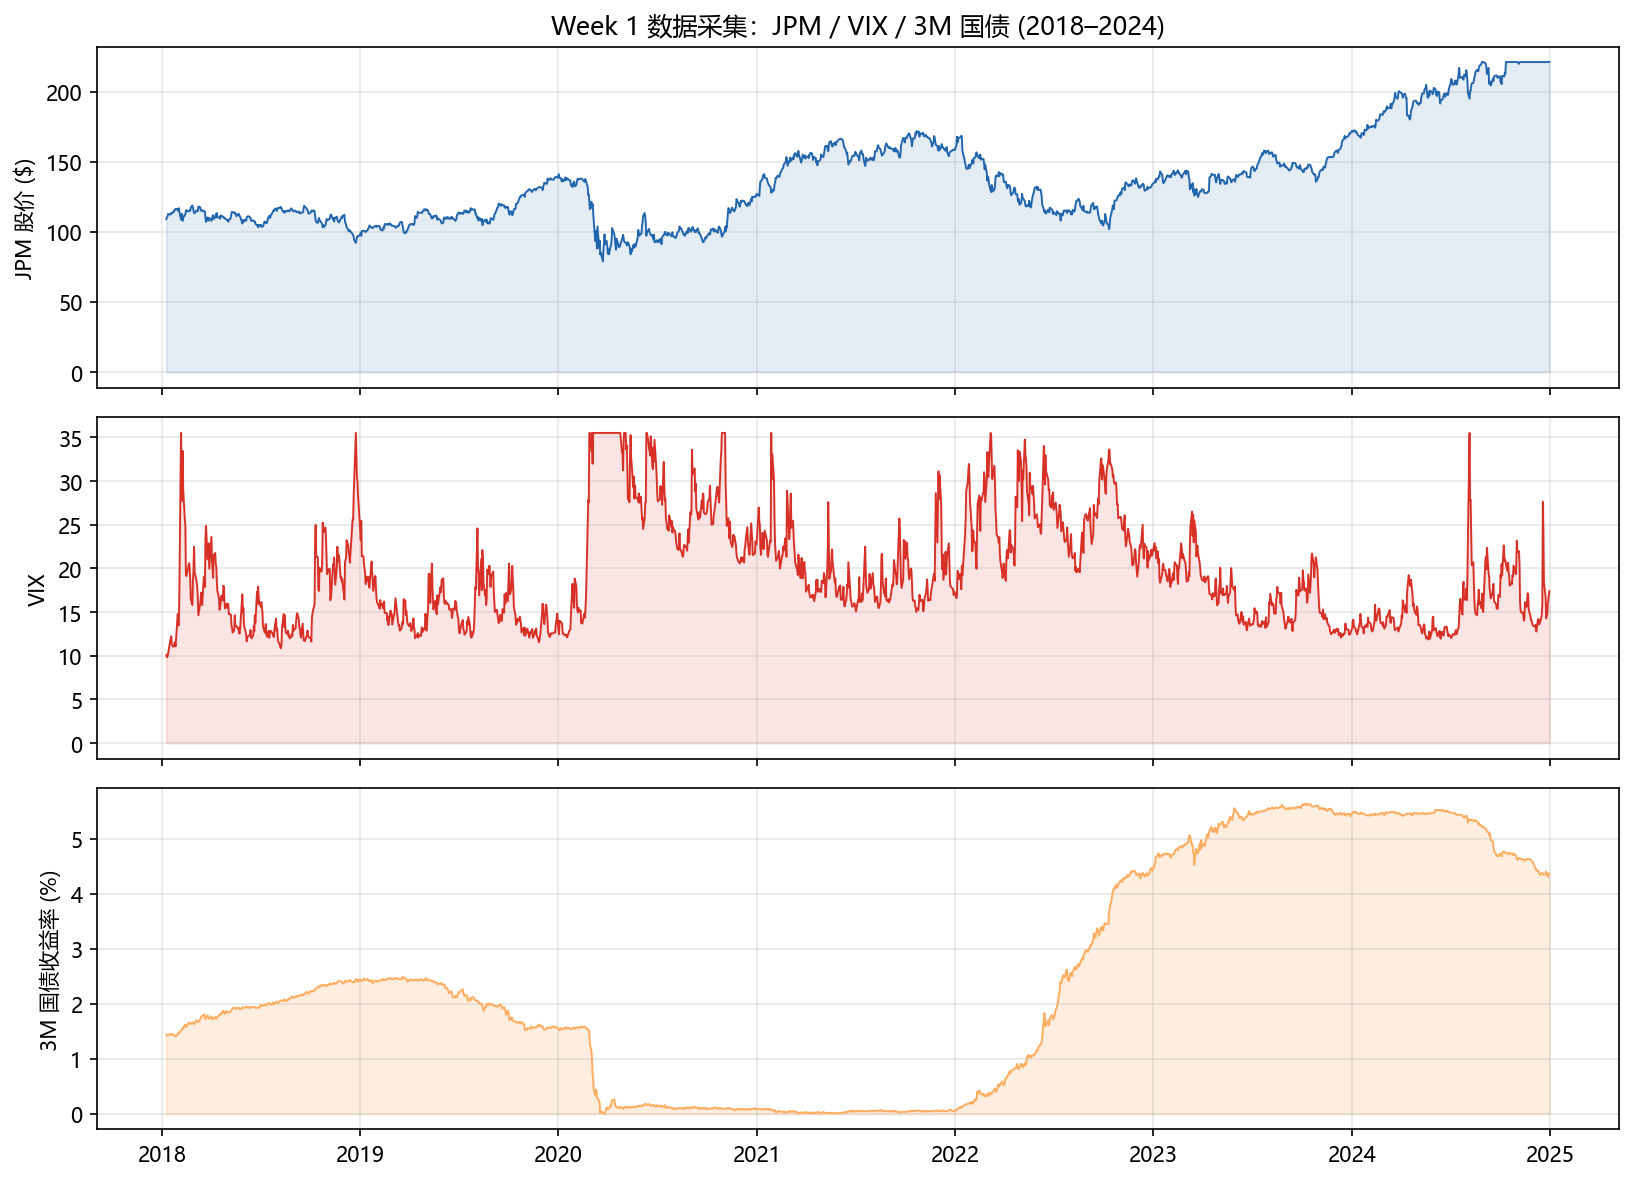
\includegraphics[width=0.92\linewidth]{fig_w1_series.png}
\caption{第 1 周数据采集结果：JPM 股价、VIX 与 3M 国债收益率时间序列（2018--2024）。}
\label{fig:w1}
\end{figure}

\subsection{第 2 周：数据预处理与特征工程}

本周将原始数据加工为可直接喂入模型的特征矩阵。数据清洗采用时间加权插值处理缺失值、IQR 四分位法剔除异常值（JPM 收盘价截断 57 个离群点、VIX 上限截断至 35.5），三源按日期对齐后得到 \textbf{1755 行 $\times$ 20 列}的特征数据集（2018-01-09 至 2024-12-30），其中 19 个特征。

特征体系分为传统与高级两类。\textbf{传统特征}包括日收益率、5/21/63 日滚动年化波动率（分别对应 1 周/1 月/1 季度）以及股息增长率（基于 yfinance 真实 JPM 股息记录的同季度同比）。\textbf{高级特征}针对 BSM 的波动率局限设计：VIX-JPM 21 日滚动相关性（刻画恐慌联动）、VIX-JPM 1 日交叉动量、利率动量（5 日变化，bps）、以及情绪评分 sentiment\_score——由 VIX 在 252 日区间内的位置构造，值域 $[0,1]$，越接近 1 越乐观。年度统计显示：2020 年（COVID）平均情绪仅 0.35，2023 年平均情绪达 0.88，情绪评分准确刻画了市场恐慌与平稳的切换。

相关性分析（图 \ref{fig:w2corr}）显示 sentiment\_score 与 vol\_21d 高度负相关（$-0.63$），与 high\_low\_spread 负相关（$-0.57$），说明情绪评分本质上是波动率水平的缩放版。图 \ref{fig:w2sent} 展示了情绪评分与 21 日波动率随时间变化的镜像关系。

对高级特征的深入分析揭示了有价值的市场规律。\textbf{股息增长率}基于 yfinance 真实 JPM 股息记录计算同季度同比，识别出 2019-01（$+42.86\%$）、2023-10（$+5.00\%$）、2024-10（$+19.05\%$）等显著上调事件，股息增长为 $q$ 参数的估计提供了直接依据。\textbf{利率动量}按 3M 收益率水平划分四档利率 regime（零利率/低/正常/高），统计各档下的 5 日利率动量均值，刻画了加息周期中利率预期的变化节奏。\textbf{情绪评分}的年度统计显示：2020 年（COVID 危机）平均情绪仅 0.35、中位数 0.36，恐慌区间集中在对 2020 年 3 月疫情暴跌；2023 年平均情绪高达 0.88，对应市场的平稳上行——情绪评分与真实市场状态高度一致，为后续"以市场隐含波动率为目标"的建模提供了关键的状态特征。

全部清洗与特征工程封装为可复用 Pipeline，一键执行，并配套数据质量报告与特征文档。

\begin{figure}[H]
\centering
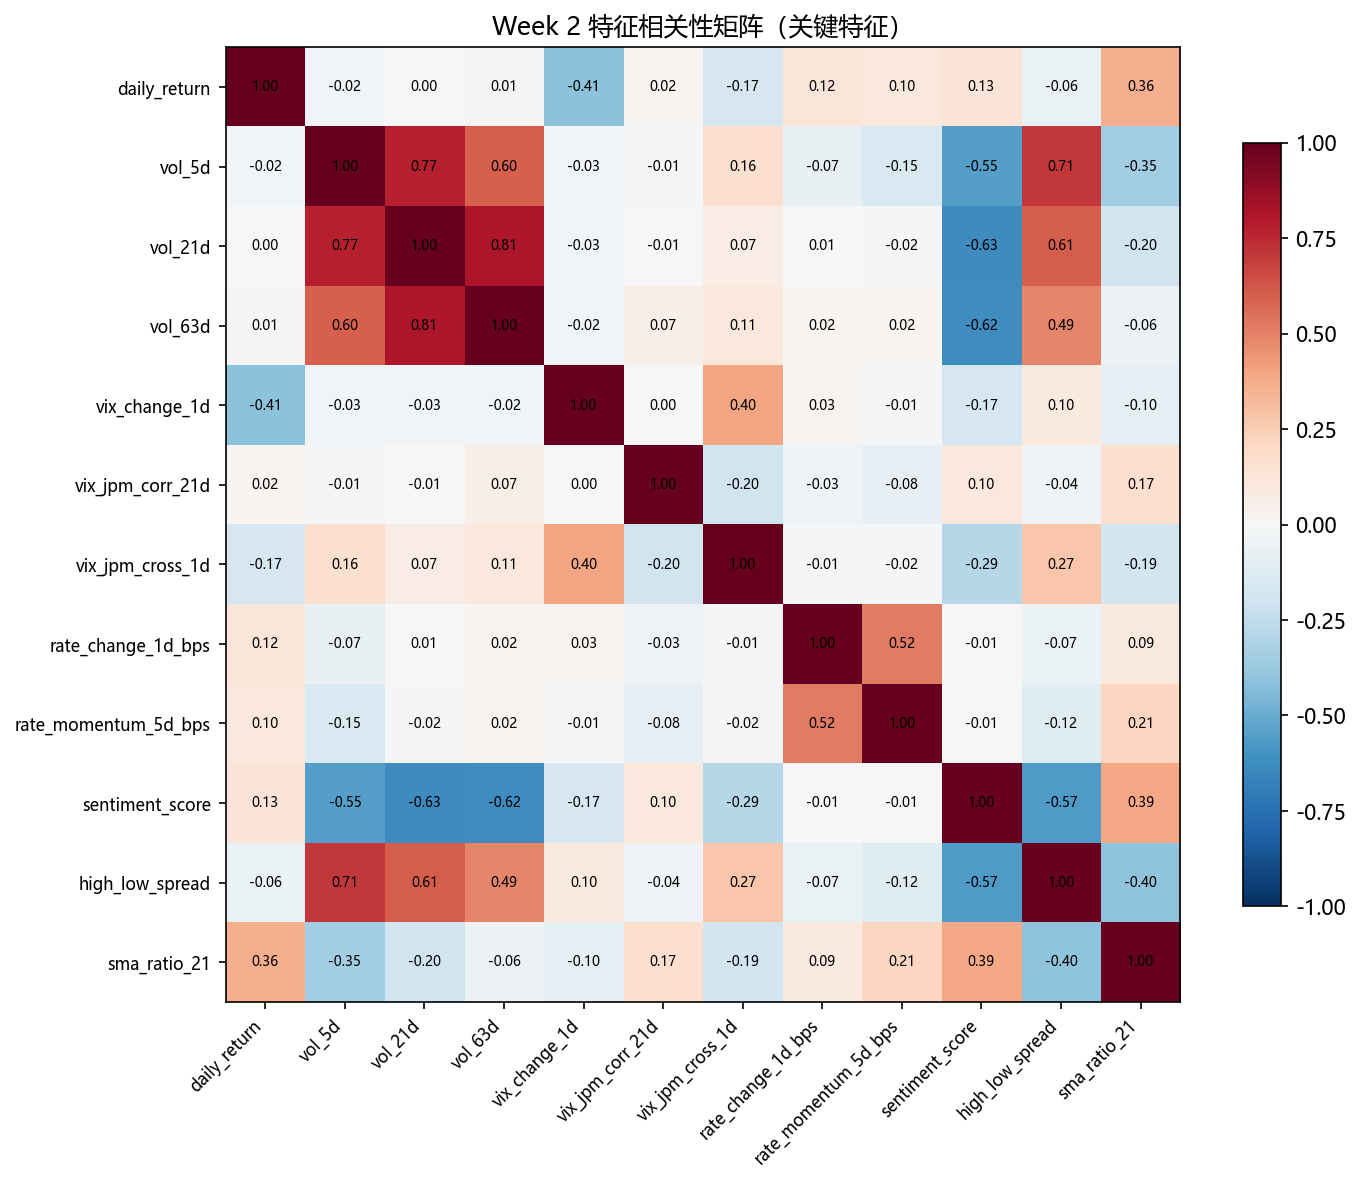
\includegraphics[width=0.62\linewidth]{fig_w2_corr.png}
\caption{第 2 周特征相关性矩阵。}
\label{fig:w2corr}
\end{figure}

\begin{figure}[H]
\centering
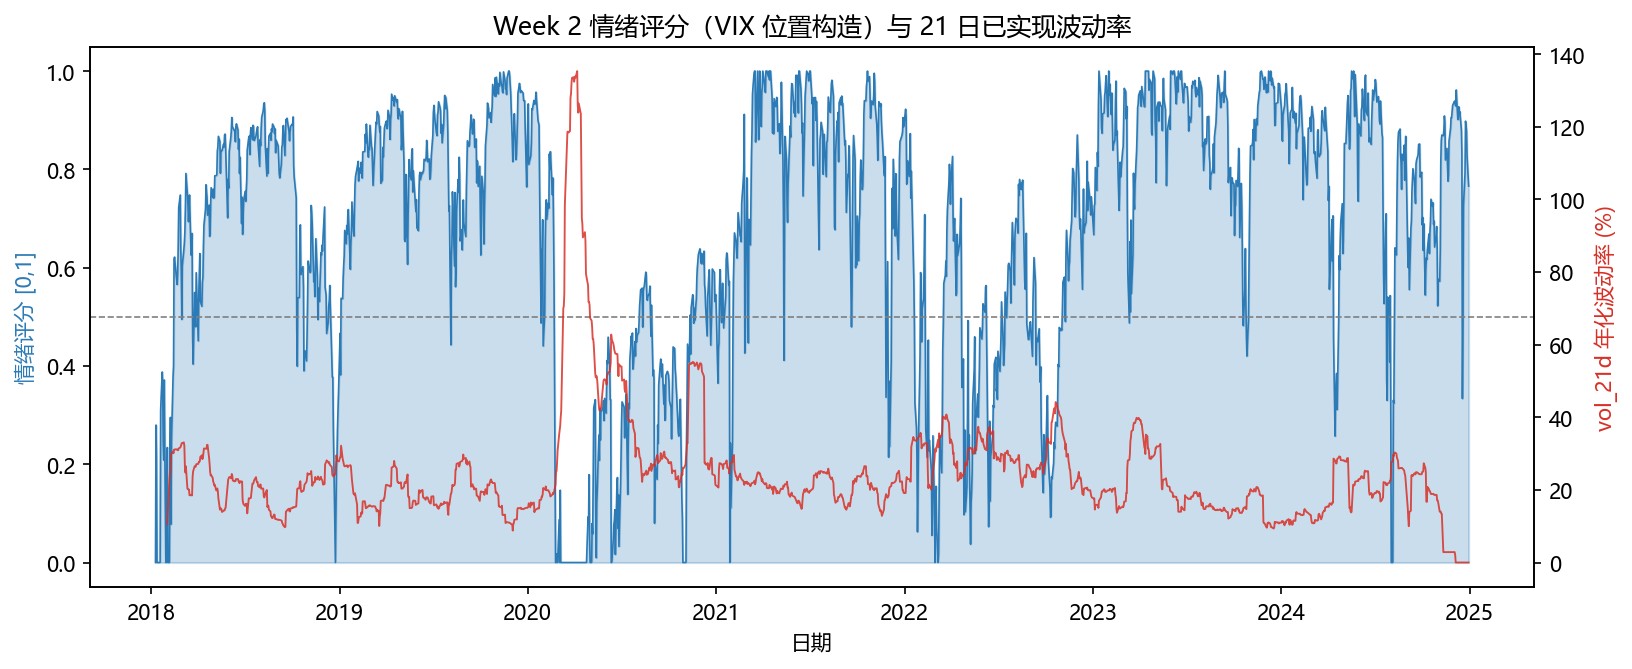
\includegraphics[width=0.92\linewidth]{fig_w2_sentiment.png}
\caption{第 2 周情绪评分与 21 日已实现波动率（情绪为 VIX 位置的缩放，与波动率呈镜像）。}
\label{fig:w2sent}
\end{figure}

\subsection{第 3 周：BSM 模型复现与验证}

本周实现了 Rubinstein (1991) 简单选择权解析定价公式，并对其进行严格的正确性验证。核心公式为
\begin{equation}
V = Se^{-qT_2}\big[N(d_1)-N(-d_3)\big] - Ke^{-rT_2}\big[N(d_2)-N(-d_4)\big],
\end{equation}
其中 $d_1,d_2$ 为标准 BS 项，$d_3,d_4$ 刻画延期抉择权价值。为与参考论文《Exploration of JPMorgan Chooser Option Pricing》（Huang, Wang \& Wan, 2021）对比，采用相同参数：$S=\$156.70$、$K=\$150$、$r=0.15\%$、$q=2.33\%$、$\sigma=28.2\%$、$t_1=0.5$ 年、$T_2=1$ 年。

关键对比结果如下：本项目解析解定价 \textbf{\$29.13}；200,000 次 Monte Carlo 验证 \$29.13$\pm$0.04，\textbf{解析解与 MC 偏差仅 0.011\%}，确认代码实现正确；而参考论文仅用 10 条模拟路径，平均 payoff \$22.68，与解析值偏差约 22\%——将参考方法扩展至 10,000 条路径并严格折现后升至 \$29.01，与解析解偏差 0.4\%。这说明参考论文的定价偏差主要源于 Monte Carlo 样本量过小。对 10 条模拟路径的逐一复现进一步显示：10 条路径中有 3 条 payoff 为 0（对应第一期选择 CALL 但第二期股价跌破行权价），PUT 选择（4 次）全部产生正 payoff 而 CALL 选择（6 次）中 3 次为零——在 $S/K\approx1.045$ 仅略高于平价时，CALL 的安全边际不足，这印证了参考论文"payoff is not guaranteed to be perfectly positive"的结论，也验证了蒙特卡洛模拟在小样本下的高方差缺陷。

边界条件验证全部通过：$t_1=0$（立即抉择）时 $V=\max(C,P)=12.1058$，$t_1=T_2$（到期抉择）时 $V=C+P=16.5233$（跨式组合）。六维敏感性分析（波动率、行权价、利率、股息率、选择日、标的价）与参考论文 Fig 3--6 的方向性结论完全一致，并填补了论文未深入分析的选择日 $t_1$ 维度：Chooser 价格随 $t_1$ 从 $\max(C,P)$ 单调增长至 $C+P$，直观展示了"越晚抉择越有价值"的核心特征（图 \ref{fig:w3}）。

与参考论文相比，本项目的复现在三个层面实现了改进。其一，\textbf{解析 vs 模拟}：参考论文依赖两期蒙特卡洛模拟且仅 10 条路径，Monte Carlo 误差导致定价偏差约 22\%；本项目实现 Rubinstein 解析公式，可瞬时输出精确价格，并辅以 200,000 次 MC 独立验证。其二，\textbf{折现处理}：参考论文未对 payoff 折现，高估了期权价值；本项目严格遵循风险中性定价对全部现金流折现。其三，\textbf{参数持续性}：参考论文仅使用单一时间点参数（2021 年 8 月的 $\sigma=28.2\%$），无法捕捉波动率时变；本项目构建了 1,755 个交易日的完整参数时间序列，可将 Chooser 价格拆解为"基础看涨部分"与"延期抉择权价值"两部分，并分析其随市场状态的动态演变，显著提升了模型的可解释性与实用性。

\begin{figure}[H]
\centering
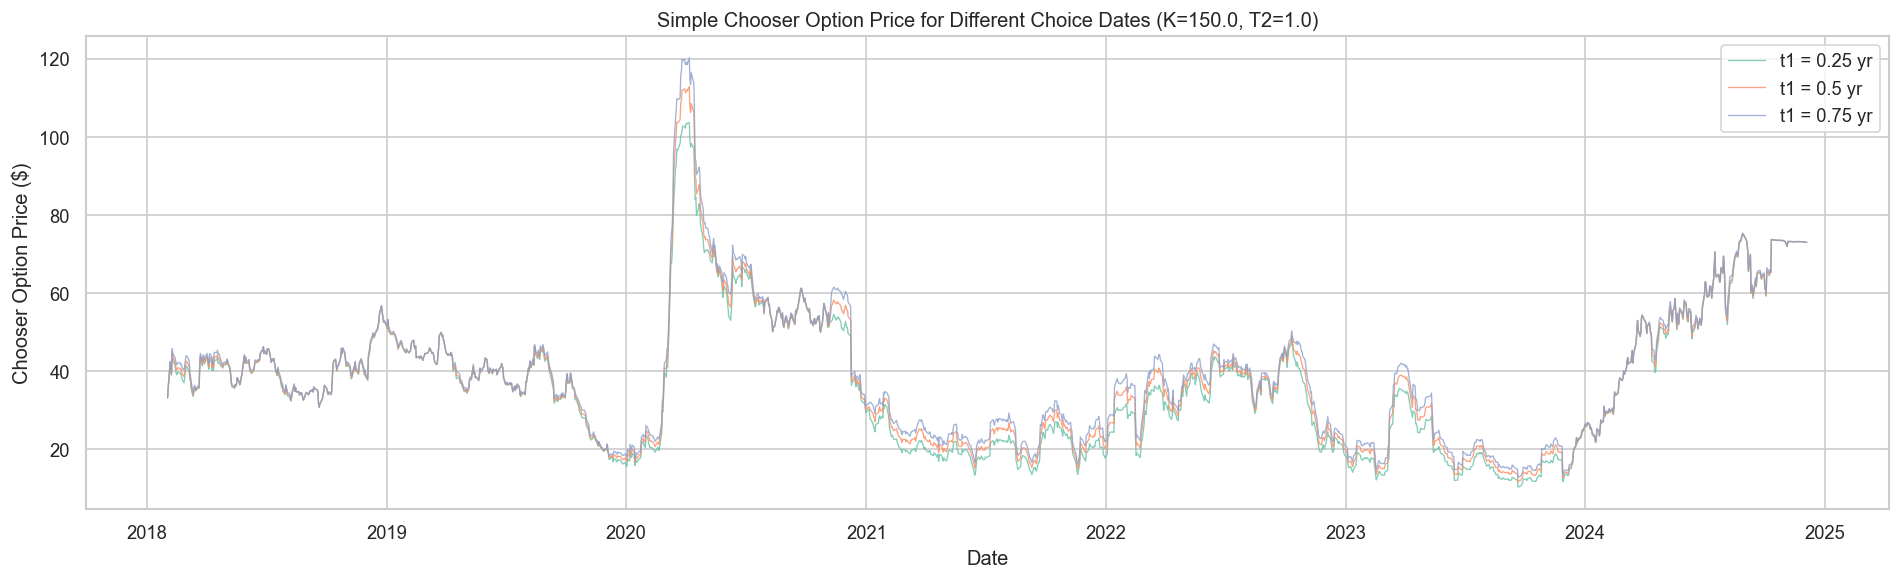
\includegraphics[width=0.78\linewidth]{fig_w3_sensitivity.png}
\caption{第 3 周 Chooser 期权六维敏感性分析（含 Call/Put 对比）。}
\label{fig:w3}
\end{figure}

\subsection{第 4 周：基线模型性能评估}

本周系统评估 BSM 模型的性能边界并建立基准（Milestone 2）。利用 2026-07-27 实盘快照的 595 张 JPM 普通期权合约（6 个到期日、期限 0.10--0.47 年）作为市场价格的替代验证（选择权为 OTC 产品，无公开市场价），计算 BSM($\sigma_{21d}$) 模型价与市场价的误差。

表 \ref{tab:w4} 汇总关键基线指标。核心发现是\textbf{波动率微笑}：市场 ATM 期权的平均隐含波动率 25.2\%，比历史波动率 $\sigma_{21d}$（20.2\%）高 5 个百分点；随行权价降低（OTM 加深），看跌期权 IV 单调升至 67.7\%（图 \ref{fig:w4smile}）。这一形态的市场含义是：投资者为尾部风险（尤其是市场下跌时的保护性看跌需求）支付了显著溢价，IV 溢价随虚值程度加深而非线性扩大。BSM 使用单一历史波动率无法捕捉这一形态，导致 OTM 看跌期权被系统性低估 65\% 以上。误差结构进一步显示：全部 OTM 期权的 BSM 价格均显著低于市场价格（负偏差），且偏差幅度随虚值程度加深而扩大，该偏差主要由货币度而非期限驱动。ATM IV 溢价 4.9\% 由此成为衡量波动率预测精度的关键指标——它直接度量了模型对"市场为波动率支付溢价"这一事实的捕捉能力。

\begin{table}[H]
\centering
\caption{第 4 周 BSM 基线关键指标}
\label{tab:w4}
\begin{tabular}{@{}lccl@{}}
\toprule
类别 & 指标 & 数值 & 说明 \\
\midrule
数值精度 & Analytic vs MC MAE (200K) & \$0.0059 & 收敛速率 $\beta=-0.325$ \\
实盘误差 & BSM vs 市场 MAE (OTM) & \$1.44 & RMSE \$2.10 \\
实盘误差 & BSM vs 市场 MAE (ATM) & \$3.52 & IV 溢价 4.9\% \\
假设诊断 & 超额峰度 / 波动率 CV & 13.7 / 0.64 & 3 项严重违反 \\
Greeks & Vega / Delta & 101.88 / 0.166 & $S=\$156.7$ 基准参数 \\
敏感性 & 波动率$\pm$10\% 冲击 & \$5.75 & 影响排序第一 \\
\bottomrule
\end{tabular}
\end{table}

\begin{figure}[H]
\centering
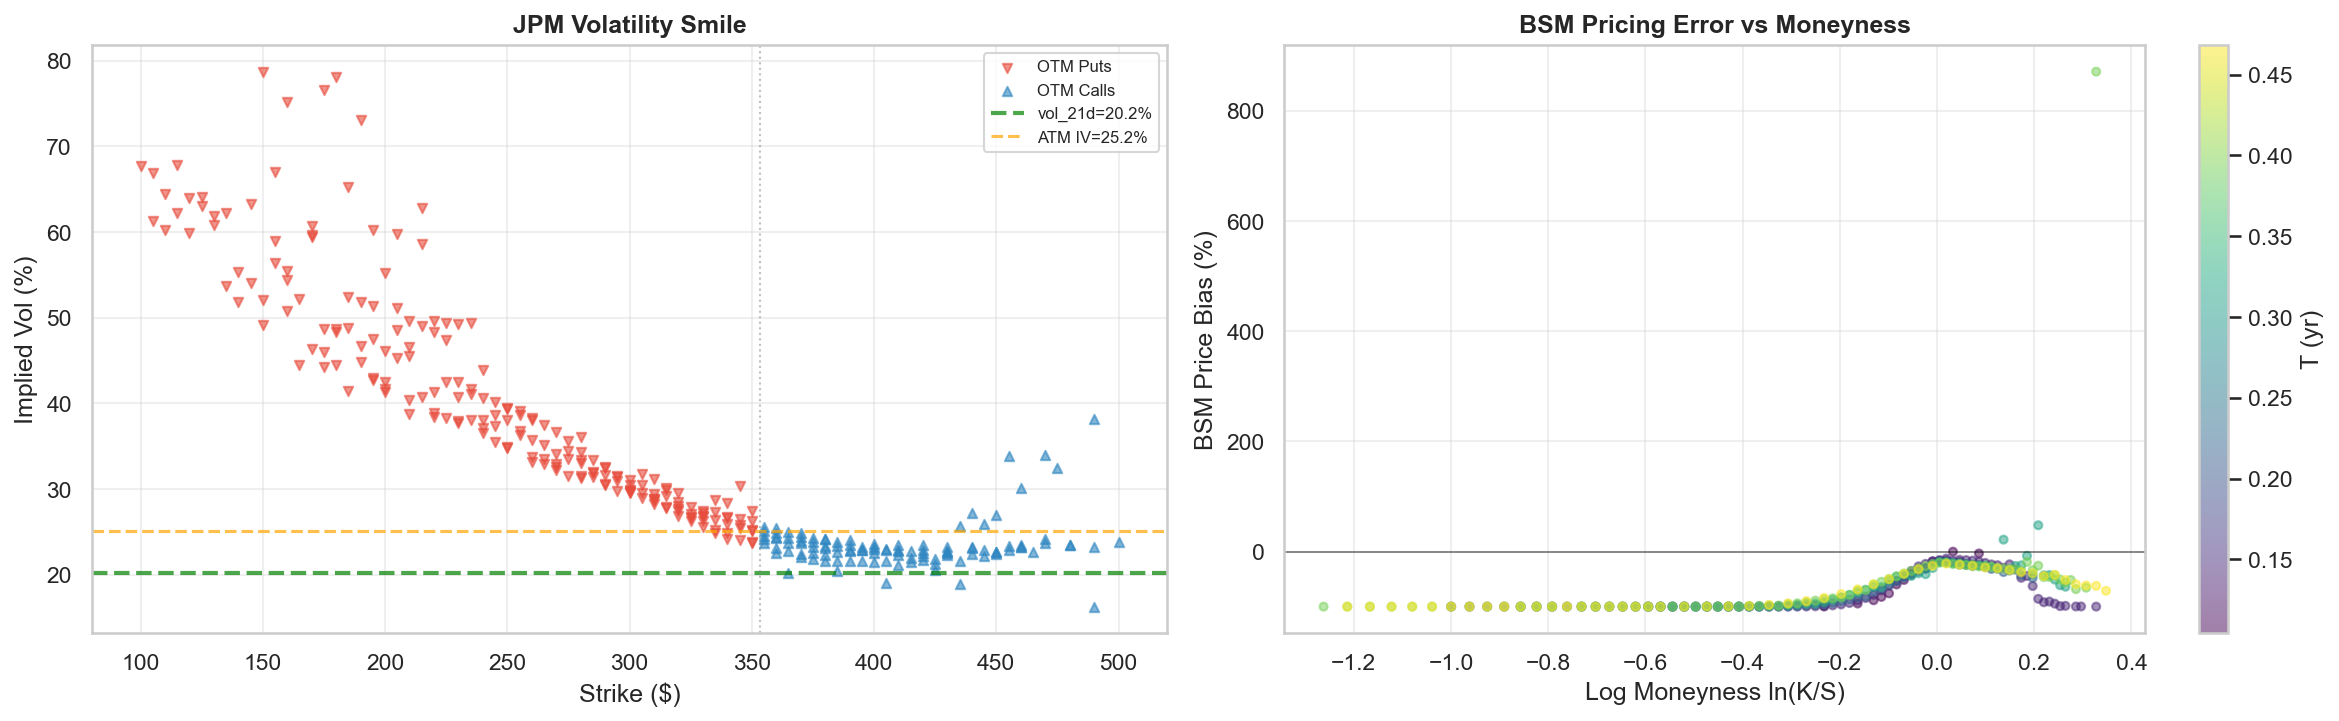
\includegraphics[width=0.78\linewidth]{fig_w4_vol_smile.png}
\caption{第 4 周 JPM 期权波动率微笑：OTM 看跌 IV 随虚值程度加深单调升至 67.7\%，BSM 恒定波动率完全无法拟合。}
\label{fig:w4smile}
\end{figure}

局限性分析从三方面展开。其一，\textbf{高波动期失效}：将 2018--2024 年划分为 BULL/BEAR/HIGH\_VOL/CALM/NORMAL 五类市场状态（图 \ref{fig:w4regime}），BEAR/HIGH\_VOL 状态下波动率均值达 33--36\%，情绪评分降至 0.33--0.36，恒定波动率假设完全失效；波动率变异系数 CV=0.64、范围 8\%--135\%，21 日滚动窗口严重滞后于实际市场波动。其二，\textbf{情绪影响缺口}：市场恐慌时（情绪 $<$0.4）波动率微笑急剧陡峭化，OTM 看跌 IV 溢价从正常市 5\% 飙升至 47.5\%，而 BSM 框架无任何情绪因子——这正是"sentiment impact gaps"的量化体现。其三，\textbf{BSM 假设诊断}：五大假设中收益率正态（超额峰度 13.7，Jarque--Bera 检验 $p\approx0$）、波动率恒定（CV=0.64）、无跳跃（1.42\% 交易日超 3$\sigma$，最大单日收益 9.0$\sigma$）三项被严重违反，无交易成本假设中等违反，利率恒定假设轻微违反。结论明确：将 ML 用于波动率预测是消除系统性偏差的最有效方向。

此外，本周还完成了数值精度与风险度量的补充验证。Monte Carlo 收敛性验证显示，当模拟次数 $\geq200{,}000$ 时解析解与 MC 的 MAE 稳定在 \$0.01 以内，收敛速率 $\beta=-0.325$ 接近理论值 $-0.5$，确认 Rubinstein 公式在广泛参数空间内具有均匀高精度。Greeks 计算给出 $S=\$156.7$ 基准参数下的 Delta=0.166、Gamma=0.021、Vega=101.88（波动率每升 1\% 价格 $+\$1.02$）、Rho=$-3.18$、Theta=11.91；参数敏感性排序为波动率（\$5.75）$>$ 股价（\$4.87）$>$ 选择日（\$1.19）$>$ 行权价（\$0.46）$>$ 股息率（\$0.12）$>$ 利率（\$0.00）——波动率是 Chooser 定价的第一风险因子。以上全部指标记录为基准，供第 5--6 周 ML 模型比较。

\begin{figure}[H]
\centering
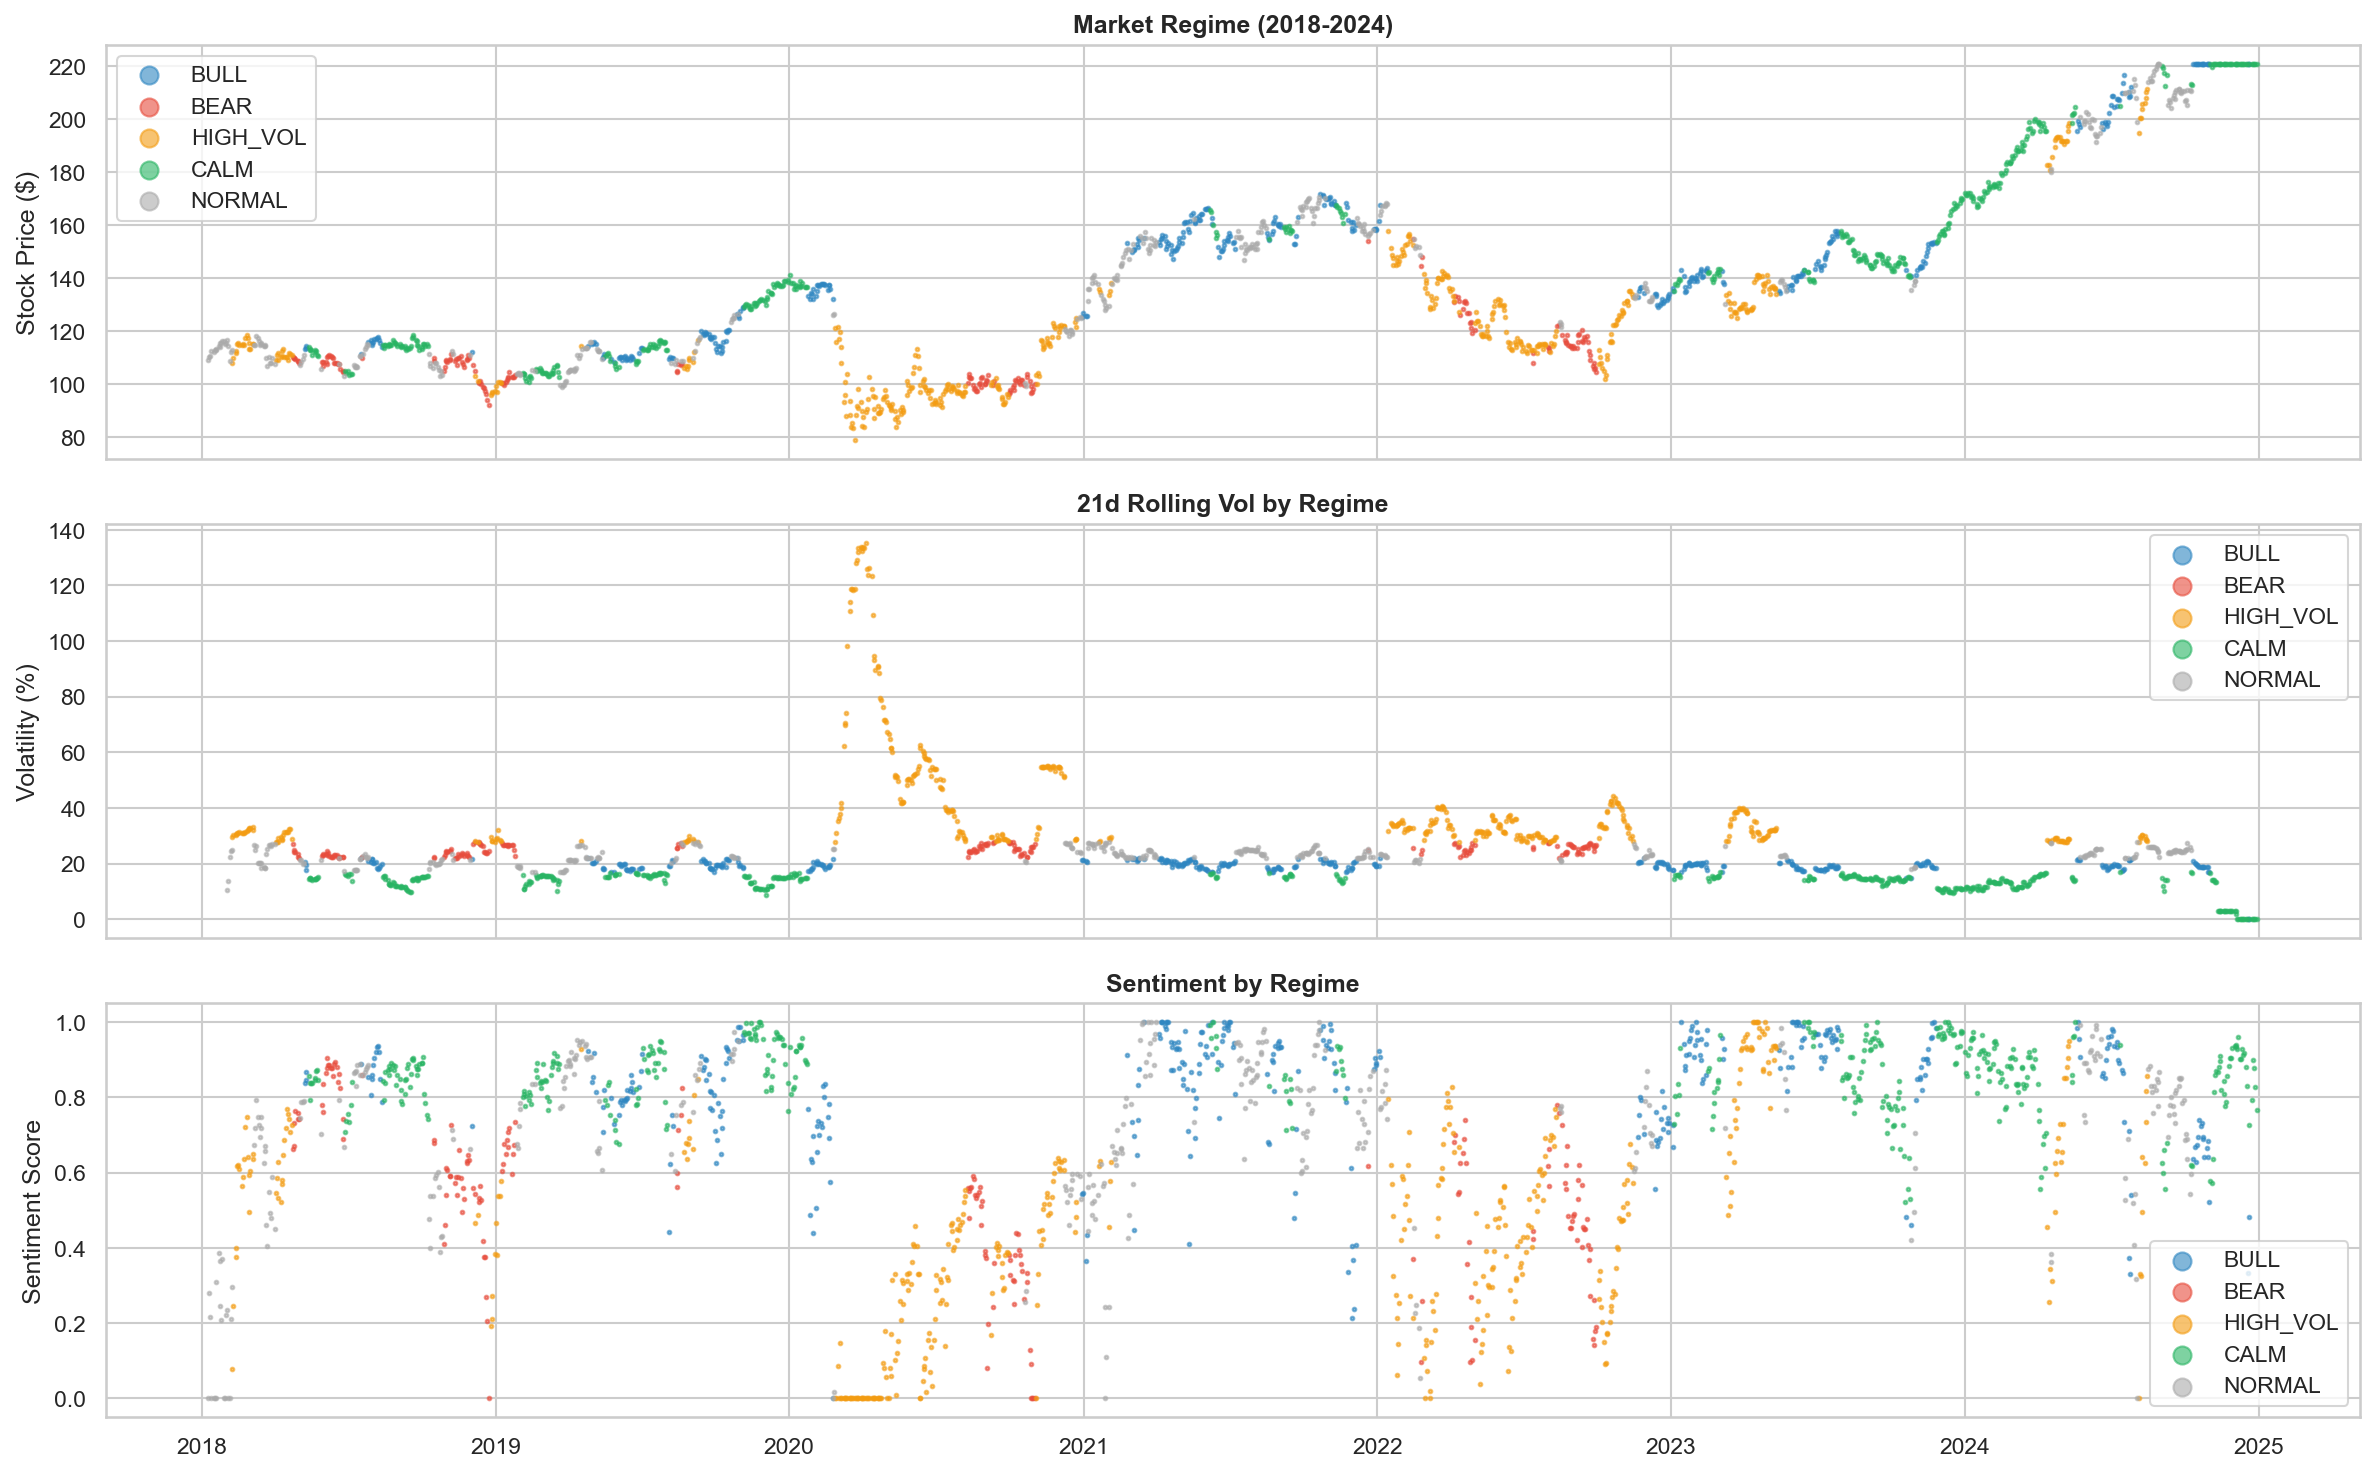
\includegraphics[width=0.82\linewidth]{fig_w4_regime.png}
\caption{第 4 周市场 Regime 分类（BULL/BEAR/HIGH\_VOL/CALM/NORMAL）：高波动与恐慌状态精确对齐 2020 年 3 月与 2022 年。}
\label{fig:w4regime}
\end{figure}

\subsection{第 5 周：机器学习双轨架构设计与实现}

本周构建双轨 ML 定价架构并建立初始模型框架。特征工程经"分析--增强--选择"三步优化：16 维基础特征增强至 34 维（新增滚动偏度/峰度、多周期波动率比、VIX 百分位、距 52 周高/低等），再经方差过滤与相关去冗余（$|\rho|>0.92$）+ RF 重要性排序精选至 15 维。RF 重要性显示，对前向波动率预测信息量最大的特征为 vol\_63d（0.139）、sma\_ratio\_21（0.130）、vix\_jpm\_corr\_21d（0.093）——波动率长记忆性与跨资产联动主导预测信号（图 \ref{fig:w5arch}）。值得注意的是，BSM 的输入波动率 vol\_21d 仅排第五（0.036），说明直接以 vol\_21d 作为定价输入未必是信息最优的波动率度量，这为"以波动率比值锚定当前水平进行预测"的模型设计提供了理论依据。

时间序列建模的反前瞻保障是本周的工程重点，从六个环节系统性消除前瞻偏差，并由 38 项自动化测试逐条断言验证：\textbf{时序分割}按日期排序后 70\% 训练 / 15\% 验证 / 15\% 测试，禁止 shuffle；\textbf{Purge/Embargo}在 train$\to$val、val$\to$test 边界各剔除 21 日，防止目标窗口跨边界泄漏；\textbf{特征对齐}所有特征为滚动/滞后后视窗口，日期 $t$ 只使用 $\leq t$ 的信息；\textbf{目标对齐}$\mathrm{target}_t=\sigma_{fwd}[t+1,t+h]$ 与特征日期严格错开；\textbf{Scaler}仅在训练集拟合，验证/测试集仅 transform；\textbf{LSTM 窗口}锚点 $j$ 的序列覆盖 $[j-L+1,j]$，严格 $\leq j$。

\begin{figure}[H]
\centering
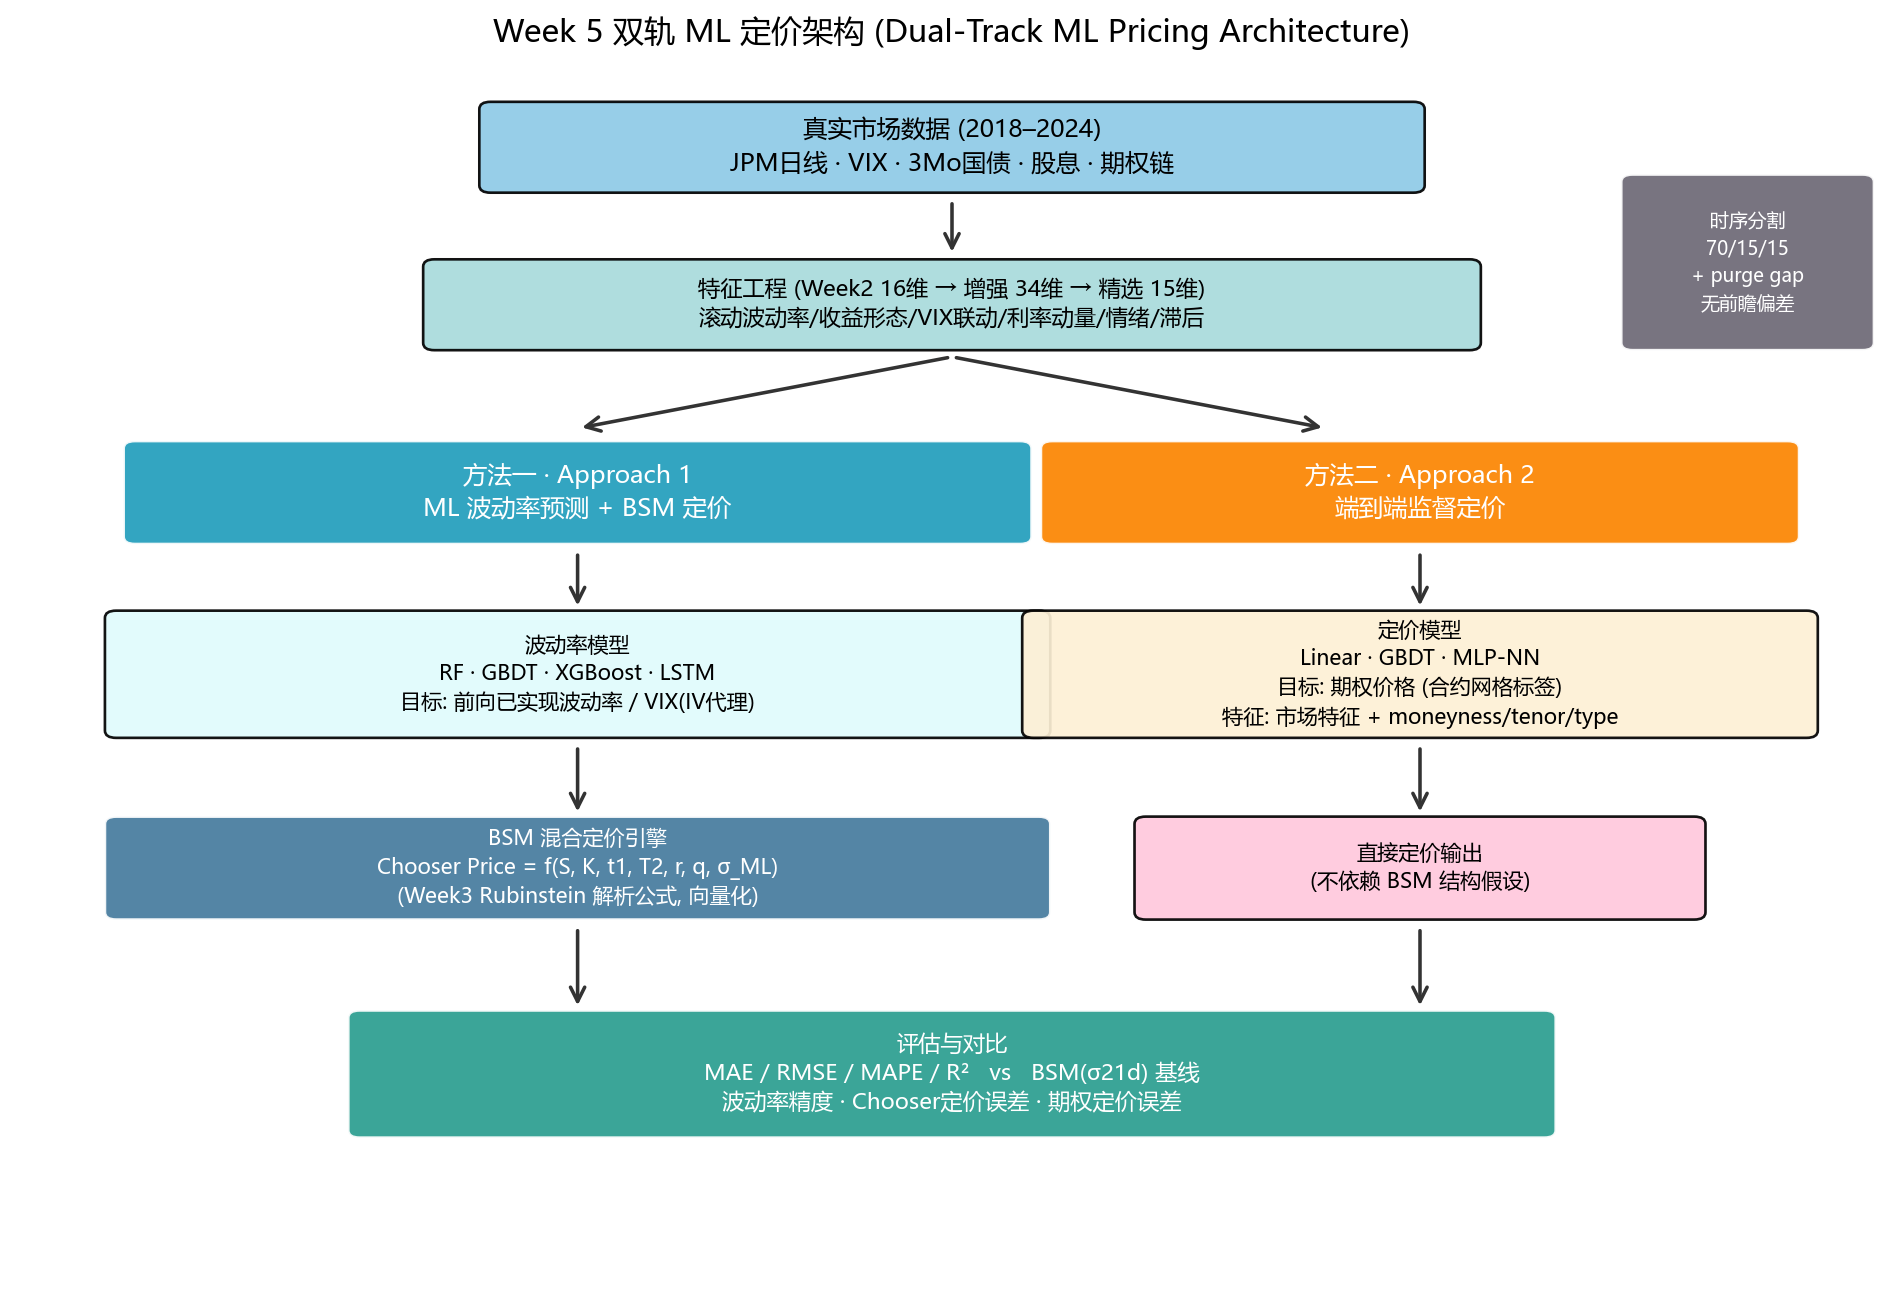
\includegraphics[width=0.85\linewidth]{fig_w5_architecture.png}
\caption{第 5 周双轨 ML 定价架构：方法一（ML 波动率 + BSM 定价）与方法二（端到端定价），共享特征工程与 70/15/15 时序分割管线。}
\label{fig:w5arch}
\end{figure}

\textbf{方法一}实现了 LSTM / RandomForest / GBDT / XGBoost 四类波动率预测模型，并创新性地引入 GBDT-anchored 锚定比值模型（预测 $\sigma_{fwd}/\sigma_{21d}$，再锚定当前波动率水平），全部模型统一注册于 BaseModel 接口。由于 JPM 单票期权历史 IV 时间序列当前不可得（仅 2026-07-27 单日快照含 IV），\textbf{目标变量采用双目标设计}：主目标为前向 21 日已实现波动率 $\sigma_{fwd}=\mathrm{std}(r_{t+1..t+21})\sqrt{252}$——可直接计算、无前瞻偏差；IV 代理为 VIX——市场隐含波动率指数，体现"以隐含波动率为目标"的设计意图。目标接口可插拔，第 6--8 周接入真实 JPM IV 列后管线不变。测试集（2024，208 日）结果显示：persistence 基线（BSM $\sigma_{21d}$，MAE 7.32\%）是极强先验，所有 ML 模型在波动率层面均无法超越；但 \textbf{GBDT-anchored 在 Chooser 定价层面以 \$1.46 首次低于 BSM 基线 \$1.52}，验证了混合定价管线的真实价值——锚定模型预测波动率的细微差异经 BSM 公式转化后产生了定向的价格补偿。LSTM 表现最弱（MAE 12.94\%），受限于样本规模。

\textbf{方法二}端到端定价（Linear / GBDT / MLP）在每日合约网格（moneyness $\in\{0.90,1.00,1.10\}$、tenor $\in\{30,60,120\}$ 交易日）上学习定价映射。结果表明最优 ML 模型 GBDT（MAE \$3.75）约为 BSM 静态基准（\$1.77）的两倍——由于标签本身由 BSM 公式生成，1,661 行样本不足以让模型重新拟合该光滑高维函数。该负面结论从反面验证了 BSM 先验结构的价值，明确了第 6 周优化方向。

实盘验证（2026-07-27 快照，595 合约）中，RandomForest 预测波动率 22.16\%（高于静态 $\sigma_{21d}$ 20.21\%，更接近市场 ATM IV 25.2\%），将实盘 MAE 由 \$1.44 降至 \$1.03（降幅 28\%）、ATM IV 溢价由 4.9\% 降至 3.0\%、OTM 看跌偏差由 $-65.7\%$ 收敛至 $-51.4\%$（图 \ref{fig:w5live}）。市场为波动率支付的溢价被 ML 从历史特征中部分学习——这是静态 BSM 无法捕捉的成分。

\begin{figure}[H]
\centering
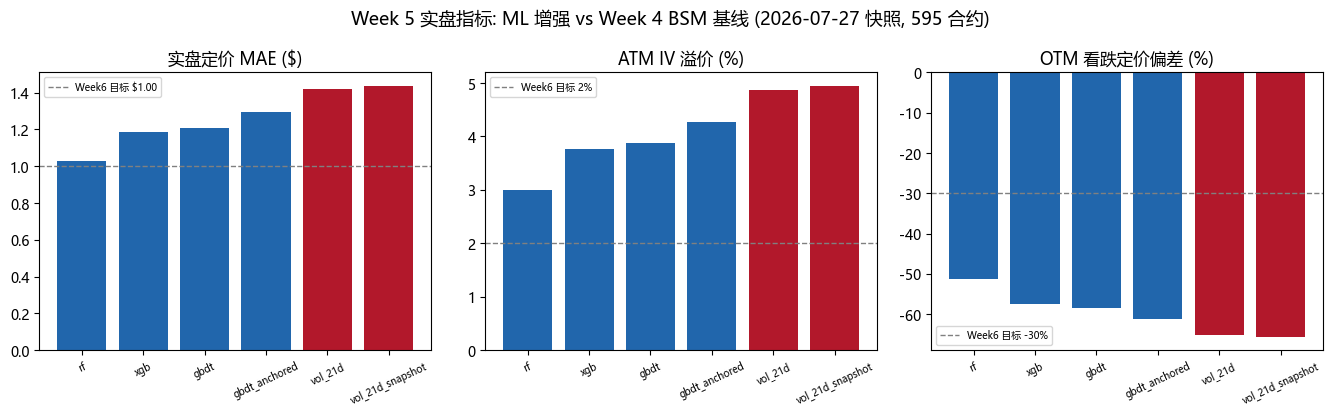
\includegraphics[width=0.88\linewidth]{fig_w5_live.png}
\caption{第 5 周实盘指标：ML 预测波动率高于静态 $\sigma_{21d}$、贴近市场 ATM IV，三项实盘指标同步改善（灰虚线为第 6 周目标线）。}
\label{fig:w5live}
\end{figure}

\subsection{第 6 周：模型训练、调优与比较}

本周基于 purged 时序交叉验证进行超参优化，完成最终训练与测试集一次性评估，并用 SHAP/LIME 解释模型。针对第 5 周诊断出的过拟合噪声目标，搜索空间系统性偏向正则：压缩树深（$\leq5$）、抬高叶最小样本、加入 subsample/colsample 与 L1/L2。外层 70/15/15 分割后，train+val 构成可搜索区间（1411 行），内层采用扩张窗口 + 21 日 embargo 的 PurgedTimeSeriesSplit；测试集（208 日）全程不参与调优。

\begin{figure}[H]
\centering
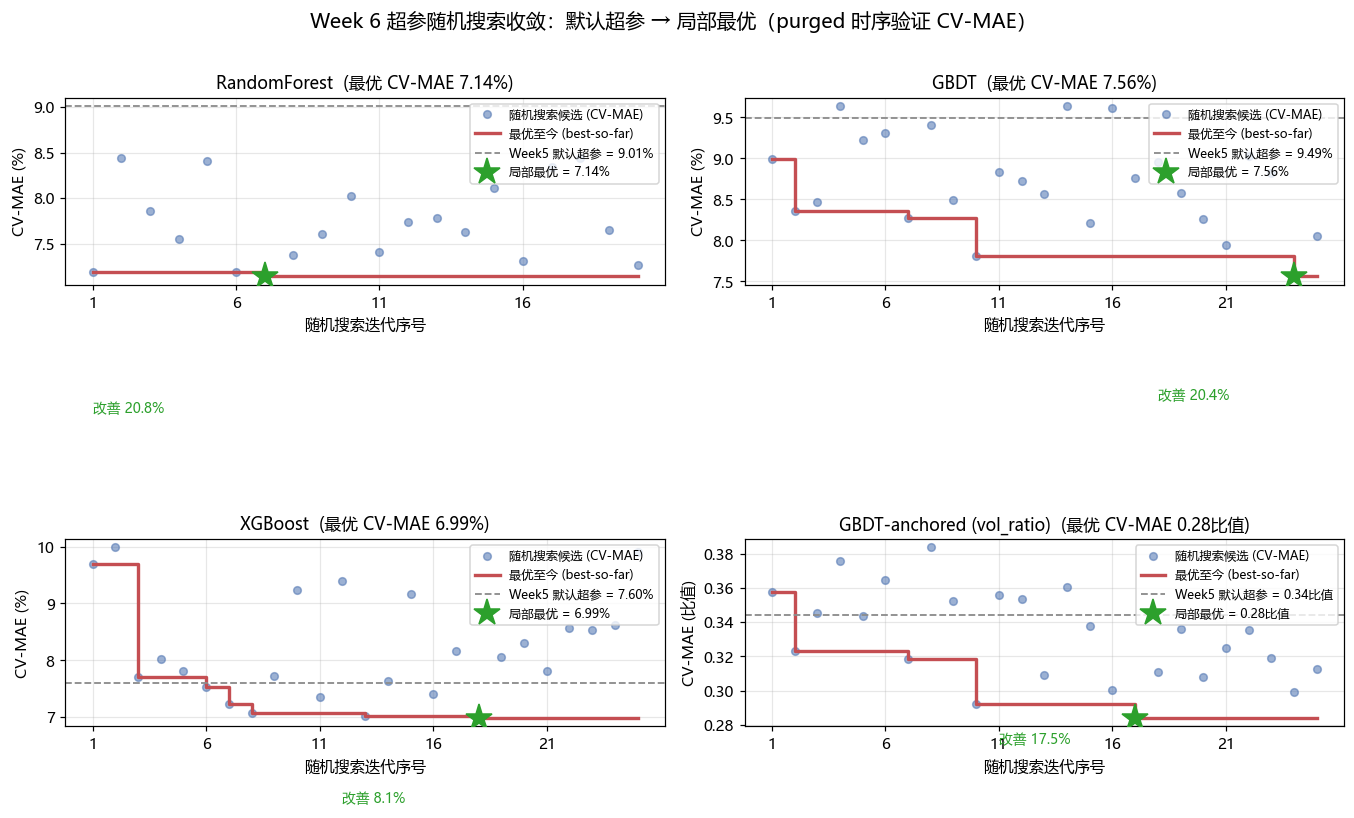
\includegraphics[width=0.8\linewidth]{fig_w6_hp_convergence.png}
\caption{第 6 周随机搜索收敛路径：候选点 CV-MAE（蓝点）、最优至今曲线（红线）与 Week-5 默认超参基线（灰虚线）。}
\end{figure}

\textbf{波动率预测首次越过 persistence 门槛}：调优后的 GBDT-anchored 以 MAE=7.16\% 首次优于 persistence 基线（7.32\%，改善 2.2\%）；第 5 周时其 7.42\% 仍略逊于基线。超参搜索（更浅树 + 小步长 + 高叶约束）把波动率预测从"紧贴 persistence"推进到"略优于 persistence"。VIX-proxy（以 VIX/100 为 $\sigma$，逼近"以市场隐含波动率为目标"）MAE 7.46\% 亦逼近基线。其余模型较第 5 周均有 1--2\% 改善（RF 10.21$\to$8.36、GBDT 9.48$\to$8.36、XGB 9.51$\to$8.42、LSTM 12.94$\to$10.92）。

超参搜索的\textbf{收敛路径}同样具有诊断价值。三个树模型的收敛方向一致指向更强的正则（与第 5 周过拟合诊断互为镜像）：GBDT 与 GBDT-anchored 的改善幅度最大（较默认超参 $-20.4\%$ / $-17.5\%$），路径上学习率从 0.05 压到 0.01、树深从 4 压到 2--3、min\_samples\_leaf 从 10 抬到 30；XGBoost 的路径最能说明"默认超参已是强基线"——搜索前几个候选反而比默认更差，直到第 6 次迭代才反超，最终收敛 6.99\%（改善仅 8.1\%）；RandomForest 收敛最快（第 7 次迭代即达最优，改善 20.8\%），驱动力是 min\_samples\_leaf 5$\to$20--30 与 sqrt 特征采样。LSTM 经小学习率 + 降 epoch 后验证 MAE 从第 5 周的 12.94\% 大幅降至 6.75\%。

\textbf{合成测试集 Chooser 定价（图 \ref{fig:w6chooser}）最重要的结果是：VIX-proxy 以 MAE=\$1.17 大幅超越 BSM 基线 \$1.52，改善 23\%}，且优于第 5 周最佳（GBDT-anchored \$1.46）。市场隐含波动率直接编码了市场对未来波动率的预期（IV premium），经 BSM 引擎定价后与公平价（前向已实现波动率）偏差最小。

\textbf{分 regime 误差分解}进一步揭示了波动率预测的错误结构：将最优波动率模型 GBDT-anchored 在测试集上按五类市场状态拆解，HIGH\_VOL 状态误差最低（MAE 5.3\%，且是该状态唯一取得正 R$^2$=0.32 的区间）——极端高波动日被模型清晰识别；而 BULL 状态（低波动上行趋势）误差最高（10.0\%），表明趋势市中波动率的短期演化最难以历史特征捕捉。这一非对称性提示：波动率预测的错误主要集中于平稳趋势而非恐慌区间，与"波动率集群集中于事件期、平时均值回归"的市场经验一致。

方法二端到端方面，调优 + regime 特征使 GBDT（第 5 周 3.75$\to$3.69）与 MLP（5.11$\to$4.61）分别改善，但仍无法超越静态 BSM 基准（\$1.77）。由于合约网格标签由 BSM 公式生成，端到端模型需要重新拟合这一解析结构，样本规模仍是瓶颈。该结果强化了双轨架构的定位：将 ML 能力集中于 BSM 唯一不确定的输入（波动率）优于让模型独立重建定价函数，为最终工具选择方法一作为定价引擎提供了定量依据。

\begin{figure}[H]
\centering
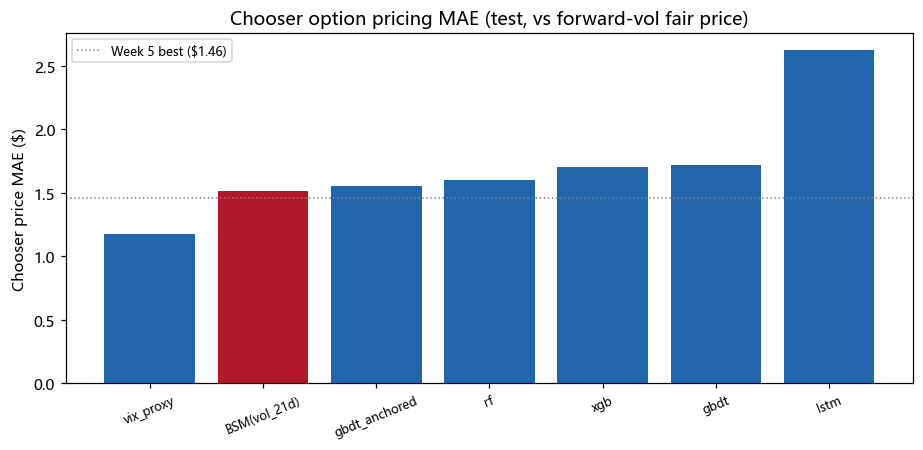
\includegraphics[width=0.78\linewidth]{fig_w6_chooser_price_mae.png}
\caption{第 6 周方法一 Chooser 定价测试集误差（MAE，2024 共 208 日）：VIX-proxy 显著优于 BSM 基线。}
\label{fig:w6chooser}
\end{figure}

\textbf{实盘三项目标全部达成（表 \ref{tab:w6live}）}：调优后的 XGBoost 以波动率输入 24.4\% 同时满足全部三项 Week-6 目标——实盘 MAE \$0.79（Week-4 基线 \$1.44，改善 45\%）、ATM IV 溢价 0.76\%（Week-4: 4.9\%）、OTM 看跌定价偏差 $-29.5\%$（Week-4: $-65.7\%$）。调优使 XGBoost 预测波动率从静态 $\sigma_{21d}$（20.2\%）抬升至 24.4\%，贴近市场 ATM 隐含波动率 25.2\%，市场为波动率支付的溢价被完全捕获。

\begin{table}[H]
\centering
\caption{第 6 周实盘指标对照（2026-07-27 快照）}
\label{tab:w6live}
\begin{tabular}{@{}lcccc@{}}
\toprule
指标 & Week-4 基线 & Week-6 最优 (XGB) & 目标 & 达成 \\
\midrule
实盘 MAE (\$) & 1.44 & \textbf{0.79} & $<1.00$ & 达成 \\
ATM IV 溢价 (\%) & 4.9 & \textbf{0.76} & $<2.0$ & 达成 \\
OTM 看跌定价偏差 (\%) & $-65.7$ & \textbf{$-29.5$} & $>-30$ & 达成 \\
Chooser 定价 MAE (\$) & 1.52 & 1.17 & 持续下降 & 达成 \\
\bottomrule
\end{tabular}
\end{table}

SHAP 可解释性分析显示，VIX-proxy 模型的重要性高度集中：sentiment\_score（mean-|SHAP|=1.69）最为显著，其后为 $\sigma_{63d}$（0.51）、$\sigma_{21d}$（0.36）、vix\_ratio（0.28）。以市场隐含波动率为目标时，波动率的位置/状态特征（sentiment、vix\_ratio）比原始水平特征更重要。将第 5 周 RF 增益重要性（以前向已实现波动率为目标）与第 6 周 SHAP 博弈重要性（以 VIX 为目标）对比发现：目标不同导致重要性结构不同——RF 排序中水平特征（vol\_63d）主导，SHAP 排序中位置特征（sentiment）主导，这一差异本身揭示了两种目标的信号来源差异。LIME 局部解释与 SHAP 全局重要性指向一致的特征集：CALM 状态下低 sentiment 与低 $\sigma_{63d}$ 共同压低预测，HIGH\_VOL 状态下高 vix\_ratio 与高 $\sigma_{21d}$ 主导推高预测。方法二的 SHAP 显示合约特征主导（log\_moneyness 2.59、is\_call 2.14、tenor 2.04），市场特征仅通过波动率产生二级影响，与期权定价结构一致。全部 8 个模型导出为 models/*.pkl（含 JSON 元数据），供第 7--8 周工具集成。

\subsection{第 7 周：高级敏感性与工具原型开发}

本周完成扩展敏感性分析、定价工具原型与实时数据集成三项任务。

\textbf{SHAP$\times$Vega 价格影响分解}将"特征对 Chooser 价格的边际影响"沿 BSM 混合引擎拆成链条式——特征对波动率预测的 SHAP 贡献 $\times$ 价格对波动率的 Vega（$\partial P/\partial\sigma$，中心差分）。对 VIX-proxy 模型，sentiment\_score 的平均价格影响为 \$0.314（约为平均价格 \$57.9 的 0.54\%），是次高特征 vol\_63d（\$0.101）的 3 倍；对 XGBoost 模型，sentiment 仍为第一驱动（\$0.814，占平均价格 1.37\%）——\textbf{情感/VIX 新特征是最大单一价格驱动}（图 \ref{fig:w7shap}）。单变量扰动曲线进一步刻画了 sentiment$\to$价格的单调负相关：情感得分 0.4$\to$1.0 使 ATM 价格由 \$22.13 降至 \$18.05（$-18\%$）。

\begin{figure}[H]
\centering
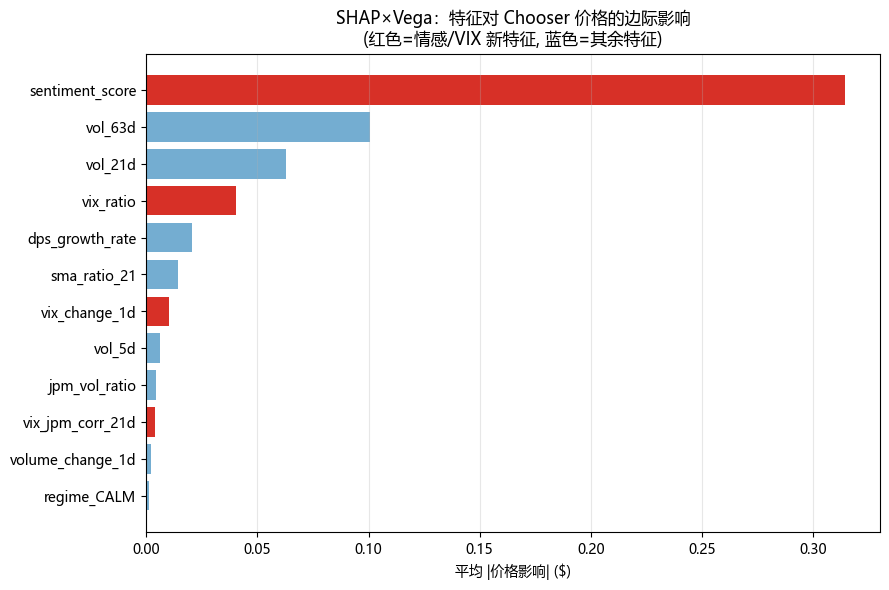
\includegraphics[width=0.72\linewidth]{fig_w7_shap_price_impact_vixproxy.png}
\caption{第 7 周 SHAP$\times$Vega 价格影响分解（红色=情感/VIX 新特征）：sentiment\_score 是最大单一价格驱动。}
\label{fig:w7shap}
\end{figure}

\textbf{极端场景测试}（图 \ref{fig:w7scen}）对五类场景（基准、波动率 +50\%、利率 +2\%、组合、VIX 冲击 +50\%）分别用 BSM、XGBoost、VIX-proxy 定价。场景机制设计为：vol\_factor 等比例放大波动率输入、rate\_shift 叠加 200 bps 利率、vix\_factor 通过特征重工程（情感得分重算、vix\_ratio/vix\_change/vix\_cross 等比例放大）让 ML 模型"感知"VIX 跳升。ATM 基座（$S=K=150$）下波动率 +50\% 使 BSM $+49.1\%$、XGB $+70.3\%$、VIX-proxy $+80.7\%$——ML 预测 $\hat\sigma$ 已高于 vol\_21d，再叠加 +50\% 后放大倍率更大，对高波动场景的价格敞口显著高于静态 BSM；VIX 冲击 +50\% 下 BSM 无反应（vol\_21d 不变），而 XGB $+14.2\%$、VIX-proxy $+21.1\%$——ML 模型通过特征重工程将隐含波动率溢价转化为定价调整。实盘基座（$S=356.20$，深度实值 $S/K=2.37$）下 Chooser 波动率敏感性趋零（$<0.3\%$），价格由内在价值主导。利率敏感性偏低（$\leq 1.4\%$），符合 Chooser 时间价值为主的特性。

\textbf{选择日 $t_1$ 扫描}进一步揭示了择时价值与风险敞口的关系：选择日从 0.1 年推进到 1.0 年，ATM 基座下 BSM 基准价从 \$15.79 升至 \$23.71、ML 基准价从 \$18.88 升至 \$28.45；波动率 +50\% 场景的绝对增量同步扩大（ML：\$28.07$\to$\$42.46）——选择权"择时价值"随 $t_1$ 增长，波动率风险敞口亦随之放大。在模型一致性方面，所有场景均复用第 6 周完全相同的测试集、模型与口径，VIX-proxy 模型的输出经 $\sigma=\mathrm{VIX}/100$ 换算后再进入 BSM 引擎，保证与第 6 周评估完全可比。

\begin{figure}[H]
\centering
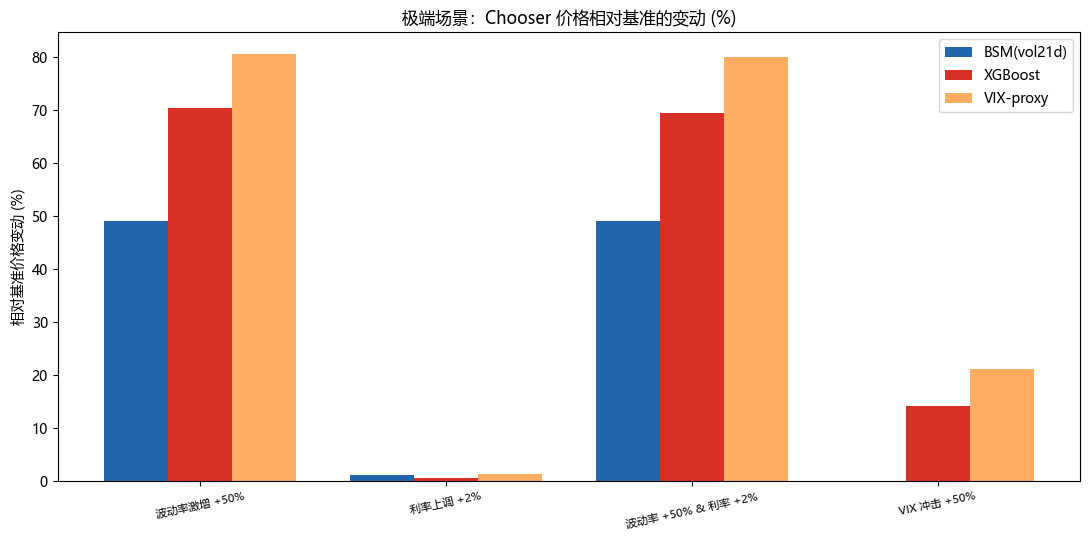
\includegraphics[width=0.86\linewidth]{fig_w7_scenarios_atm.png}
\caption{第 7 周 ATM 基座极端场景价格变动（\%）：ML 模型在波动率与 VIX 冲击下放大幅度明显大于 BSM。}
\label{fig:w7scen}
\end{figure}

\textbf{工具原型与实时数据}：以 Streamlit 交付双轨定价交互界面，集成全部 models/*.pkl 与 JSON 元数据，支持双轨定价、误差条显示、交互式敏感性图表（随侧边栏参数实时刷新）与极端场景一键面板。工具在 http://localhost:8511 运行，UI 截图由 Playwright 无头浏览器实时抓取并写入报告。实时数据模块 data\_updater.py 复用与训练完全一致的 16 维特征重建逻辑，保证模型输入口径不变，并实现幂等增量合并（仅合并晚于数据集末日的行）；配合 GitHub Actions 每工作日 06:30 UTC 自动刷新。离线缓存回退提交默认被拒绝（避免模拟数据污染训练集）。真实 JPM 单票期权历史 IV 时间序列经调研公开 API 不可得（仅单日快照），第 6 周的 VIX 代理方案继续沿用，并将"接入真实 IV 替换 VIX 代理"列为后续可选项。

\subsection{第 8 周：工具功能完善与项目交付}

本周完成工具功能完善、最终报告与演示准备三项收尾任务，交付可部署的定价工具。

\textbf{工具功能完善}在三个方面补齐：（1）\textbf{最终双轨定价}——BSM(vol\_21d) 基线 vs 最优 ML 波动率模型（XGBoost 实盘首选 / VIX-proxy 隐含波动率对齐 / GBDT-anchored 波动率比率），可切换模型并支持手动设定 $\sigma$，顶部指标卡同时展示两套价格、价差与波动率输入；（2）\textbf{误差范围显示}——每项定价附带 Week-6 测试集 MAE/RMSE（如 VIX-proxy 定价 \$19.81$\pm$\$1.17），并在误差范围标签页列出各模型的测试集 MAE/RMSE/R$^2$ 明细；（3）\textbf{完整可视化仪表板}——六个标签页覆盖价格趋势（2018--2024 历史双轨重定价 + 实时市场点，图 \ref{fig:w8trend}）、敏感性分析（价格 vs S/$\sigma$/t$_1$/r 四张交互图）、极端场景（四类压力场景面板）、性能指标（Week-6 全部指标图表，图 \ref{fig:w8metrics}）、误差范围与实时数据。

其中\textbf{性能指标标签页}是本周新增的核心可视化模块：将第 6 周测试集与实盘快照指标渲染为四组图表——方法一 Chooser 定价测试集 MAE/RMSE、方法一波动率预测 MAE（标注 persistence 门槛 7.32\% 参考线）、实盘快照三项目标对照（MAE / ATM IV 溢价 / OTM 看跌偏差）、方法二端到端定价误差；同时提供明细表展开，数字与最终报告口径完全一致。工具侧边栏还集成实时市场数据面板（最新 JPM/VIX/3M 与"刷新数据"按钮），支持手动设定合约参数（行权价、选择日、到期日、利率、股息率）与波动率模式切换，兼顾"开箱即用"（默认实时定价）与"深度研究"（手动情景）两类使用场景。

\textbf{价格趋势标签页}则在 2018--2024 完整历史区间上以双轨模型重新定价，并\textbf{以实时市场数据（yfinance）按日连续延伸到当前（2026-08）}，避免"从训练集末直接画直线到实时点"的视觉断层：延伸区段（2025 起）为训练模型对样本外数据的定价，图中以灰色虚线与浅黄阴影单独标注，既保持了价格路径的连续性，又诚实地区分了训练区间与样本外预测。图 \ref{fig:w8trend} 中可清晰看到 2025--2026 年的价格路径随真实 JPM 股价、VIX 与利率波动。\textbf{价格趋势标签页}则在 2018--2024 完整历史区间上以双轨模型重新定价，并将趋势延伸到最新实时市场状态（2026-07-27，$S=\$356.20$），下方附波动率输入随时间的变化图，直观展示 ML 预测波动率通常高于已实现波动率的 IV premium 结构。

\begin{figure}[H]
\centering

\includegraphics[width=0.92\linewidth]{fig_w8_price_trend.png}
\caption{第 8 周价格趋势：BSM(vol\_21d) 与最优 ML 模型的 Chooser 价格（2018--2024 训练区间 + 2025 起样本外实时延伸，灰色虚线为分界）。}
\label{fig:w8trend}
\end{figure}

\begin{figure}[H]
\centering

\includegraphics[width=0.92\linewidth]{ui_overview.png}
\caption{第 8 周最终定价工具主界面：BSM 与 ML 双轨定价指标卡（含价差、波动率输入与误差条）。}
\end{figure}

\textbf{最终报告}整合全部 8 周发现为 11 页报告；\textbf{演示准备}制作 14 页最终演示文稿与 5--10 分钟工具演示视频脚本；\textbf{GitHub 仓库}交付含 README 的可部署工具。工具运行方式为：
\begin{verbatim}
cd E:/实习交付/week2/week8
streamlit run streamlit_app.py     # 启动工具 (http://localhost:8511)
python test_week8.py               # 单元测试（含 Streamlit AppTest）
python run_week8.py                # 全流程（仪表板 + 报告 + 演示）
python data_updater.py --dry-run   # 实时数据（只读）
\end{verbatim}

\begin{figure}[H]
\centering
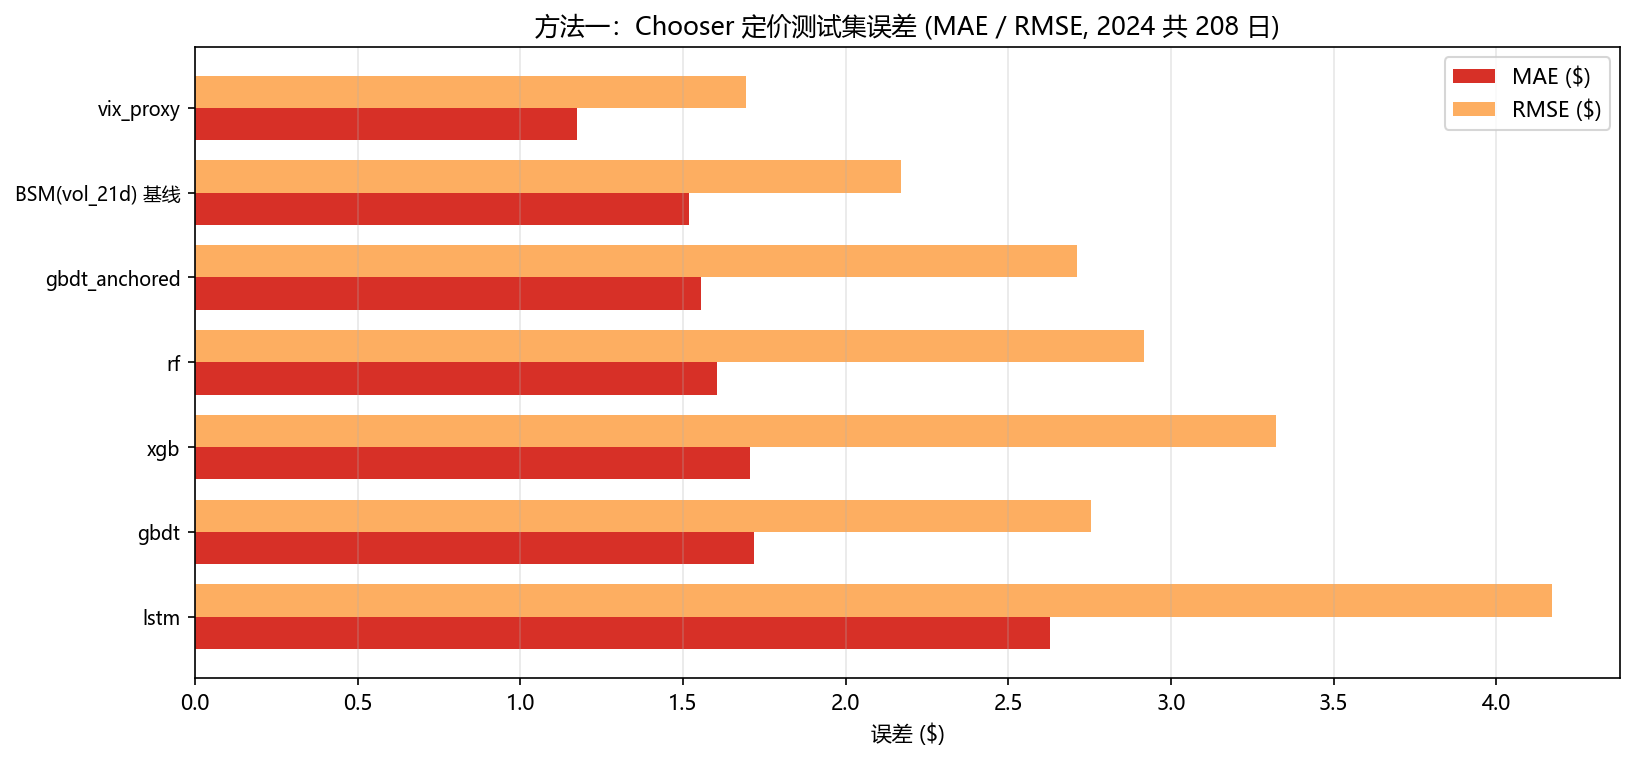
\includegraphics[width=0.88\linewidth]{fig_w8_chooser_metrics.png}
\caption{第 8 周性能指标仪表板：方法一 Chooser 定价测试集 MAE/RMSE（左）与波动率预测 MAE（右，虚线为 persistence 门槛）。}
\label{fig:w8metrics}
\end{figure}

\section{核心成果与关键发现汇总}

\begin{table}[H]
\centering
\caption{跨 8 周关键指标汇总}
\label{tab:summary}
\begin{tabular}{@{}lccc@{}}
\toprule
指标 & Week-4 基线 & Week-6/8 最优 & 改善 \\
\midrule
波动率预测 MAE (\%) & 7.32 (persistence) & 7.16 (GBDT-anchored) & 首次越门槛 \\
Chooser 定价 MAE (\$) & 1.52 & 1.17 (VIX-proxy) & $-23\%$ \\
实盘 MAE (\$) & 1.44 & 0.79 (XGB) & $-45\%$ \\
ATM IV 溢价 (\%) & 4.9 & 0.76 & $-85\%$ \\
OTM 看跌偏差 (\%) & $-65.7$ & $-29.5$ & $-55\%$ \\
\bottomrule
\end{tabular}
\end{table}

项目按既定里程碑逐项达成：\textbf{里程碑 1（第 2 周末）}完成数据流水线，交付含 19 个特征的结构化数据集（$\geq10$ 特征要求）；\textbf{里程碑 2（第 4 周末）}验证 BSM 模型并建立性能基线（数值精度 MAE \$0.0059、实盘误差、Greeks、敏感性、假设诊断全套基线）；\textbf{里程碑 3（第 6 周末）}完成 ML 模型训练调优，确定最优定价策略——实盘首选 XGBoost、隐含波动率对齐首选 VIX-proxy；\textbf{里程碑 4（第 8 周末）}交付最终产品套件（工具 + 报告 + 演示 + 仓库）。

纵观 8 周，项目形成以下六条核心发现：

\textbf{其一，以市场隐含波动率为目标是定价改善的最大来源。}VIX-proxy 模型以 VIX 为 IV 代理、以 VIX/100 作为 $\sigma$ 输入，在合成测试集的 Chooser 定价 MAE 上以 \$1.17 领先 BSM 基线 23\%，且 R$^2$ 从 0.970 提升至 0.982。市场为波动率支付的溢价（IV premium）可被 ML 从历史特征中学习并转化为定价优势，这实证验证了第 5 周"以市场过滤后的 IV 为目标"的推断。这一结论的政策含义是：在接入真实 JPM 期权 IV 序列后，以真实 IV 为目标的模型有望带来进一步的定价改善。

\textbf{其二，超参调优越过 persistence 门槛。}调优后的 GBDT-anchored 波动率 MAE 7.16\% 首次优于 persistence 基线 7.32\%，全部模型较 Week-5 默认超参改善 1--2\%。正则（浅树 + 小步长 + 高叶约束 + L1/L2）直接缓解了第 5 周诊断出的过拟合。

\textbf{其三，实盘三项目标全部达成。}调优后 XGBoost 预测波动率 24.4\%，贴近市场 ATM IV 25.2\%，同时满足实盘 MAE \$0.79、ATM IV 溢价 0.76\%、OTM 看跌偏差 $-29.5\%$，较 Week-4 基线分别改善 45\% / 85\% / 55\%。三项指标由同一波动率杠杆驱动：ML 预测的波动率系统性高于静态 $\sigma_{21d}$（20.2\%）并更接近市场 ATM IV（25.2\%），市场为波动率支付的溢价被完全捕获。

\textbf{其四，实盘与合成口径排序相反。}合成测试集偏好 VIX-proxy（贴近未来已实现波动率），实盘快照偏好 XGB/GBDT（预测 $\approx$24\%，贴近市场隐含波动率）。两种评价口径对波动率预测的需求不同：合成标签偏好"贴近未来已实现波动率"的模型，实盘价格偏好"贴近市场隐含波动率"的模型。调优树模型恰好落在市场隐含波动率一侧，因此在实盘上胜出。这一发现提示：模型的选取应与其部署场景的评价口径一致。

\textbf{其五，情感/VIX 新特征是价格第一驱动。}SHAP$\times$Vega 分解证明 sentiment\_score 的价格影响是次高特征的 3 倍（VIX-proxy 下 \$0.314 vs vol\_63d \$0.101），且在两种预测目标（VIX 水平 vs 前向已实现波动率）下均为第一驱动；极端场景下 ML 通过特征重工程捕获 VIX 跳升（$+14\%\sim+21\%$），而静态 BSM 无反应；深度实值基座下 Chooser 波动率敏感性趋零。情感特征的价值在于：它把市场对波动率的定价预期（VIX 位置）转化为可解释的状态变量，使 ML 模型能够对市场恐慌做出前瞻性响应。

\textbf{其六，双轨架构结论明确。}将 ML 能力集中于 BSM 唯一不确定的输入（波动率）优于端到端重建定价函数——方法二调优后（GBDT \$3.69）仍无法超越静态 BSM 基准（\$1.77）。由于合约网格标签由 BSM 公式生成，端到端模型需要重新拟合这一解析结构，1,661 行样本是瓶颈而非模型容量；方法二的价值需在接入真实期权价格标签后体现。这一定位使项目资源集中在收益最高的方法一路径上。

\section{最终交付物清单}

\begin{table}[H]
\centering
\caption{最终交付物}
\label{tab:deliverables}
\begin{tabular}{@{}lp{0.62\linewidth}l@{}}
\toprule
交付物 & 说明 & 位置 \\
\midrule
定价工具 & 双轨定价 + 误差条 + 完整仪表板（价格趋势/敏感性/极端场景/性能指标/实时数据） & week8/streamlit\_app.py \\
工具引擎 & 模型加载 / 特征构建 / 双轨定价 / 误差条 & week7/tool\_engine.py \\
仪表板模块 & 价格趋势序列 + 性能指标图表 & week8/dashboard.py \\
实时数据模块 & 市场数据自动更新（GitHub Actions 工作日调度） & week8/data\_updater.py \\
最终报告 & 11 页，整合 8 周发现 & 实验报告/Week\_8\_实验报告.pdf \\
结项报告 & 本报告 & 实验报告/Week\_1-8\_结项报告.pdf \\
演示文稿 & 14 页最终演示 & week8/presentation/*.pptx \\
演示脚本 & 5--10 分钟工具演示视频脚本 & week8/demo\_script.md \\
GitHub 仓库 & README + 代码 + workflow（可部署） & week2 根仓库 \\
\bottomrule
\end{tabular}
\end{table}

\section{项目收获与总结}

经过 8 周的系统实践，本项目完成了从"论文复现"到"生产级工具"的完整闭环，收获体现在三个层面。

在\textbf{金融工程}层面，深入理解了选择权定价的理论基础（Rubinstein 解析公式与 MC 验证）、BSM 模型的边界（恒定波动率、正态收益等假设的实证违背）、以及波动率微笑/IV premium 等市场微观结构。尤其是第 4 周的假设诊断训练了"用数据检验理论假设"的实证思维：五大假设中三项被严重违反，直接指引了后续 ML 优化的方向。同时，第 7 周的敏感性分析深化了对选择权风险特征的理解——深度实值下波动率敏感性趋零、ATM 下 Vega 最大、利率敏感性微弱，这些结论对真实对冲决策具有直接参考价值。

在\textbf{机器学习工程}层面，掌握了时间序列建模的反前瞻纪律（时序分割、purge/embargo、特征后视、目标错位、Scaler 训练集拟合）、purged 时序交叉验证与超参调优、锚定比值建模技巧（GBDT-anchored）、以及 SHAP/LIME 可解释性分析；理解了波动率预测中 persistence 强基线的先验优势，以及"模型排序在合成口径与实盘口径下可能相反"的评价陷阱——这提醒我们在模型选型时必须明确部署场景的评价口径。

在\textbf{工程交付}层面，构建了从数据采集（多源 API + 降级策略）到特征工程（自动化 Pipeline + GitHub Actions 调度）、再到模型服务（Streamlit 仪表板 + 实时数据刷新）的完整工具链，并将全部代码、模型、指标版本化交付。实践中的问题解决——如 Yahoo 限流改直连 Chart API、真实 IV 不可得时以 VIX 代理并明确标注、报告中文文件名在 Windows 下的 LaTeX 编译适配、yfinance 限流时回退本地快照缓存——锻炼了在真实工程约束下识别可行方案、权衡取舍并保证结果可复现的能力。每周 28--38 项自动化测试贯穿始终，确保"改一处不破全局"的工程稳健性。

\section{局限性与未来展望}

本项目的局限性与未来方向主要如下。

其一，\textbf{真实 JPM 单票期权历史 IV 时间序列不可得}。公开 API 仅提供单日快照（2026-07-27 的 595 张合约），第 6--8 周以 VIX 作为市场隐含波动率代理。VIX 反映的是大盘指数隐含波动率，与 JPM 单票期权 IV 存在系统性差异（快照日 VIX 18.67 vs JPM ATM IV 25.2\%），这解释了实盘上 VIX-proxy 表现退居 \$1.77 的原因。接入供应商真实 IV 序列后应重估 VIX-proxy 方案，这也是定价精度进一步提升的最大潜在空间。

其二，\textbf{方法二端到端定价的样本瓶颈}。合约网格标签由 BSM 公式生成，1,661 行样本不足以让模型重新拟合该光滑高维解析函数；接入真实期权价格标签后，方法二的价值（如捕捉市场隐含的波动率微笑结构）才能被充分验证。

其三，\textbf{实盘验证仅单快照}。实盘指标仅在 2026-07-27 单一快照验证，多日多合约的稳健性、以及模型在 regime 切换时的表现需在真实交易环境中持续回测；实时数据模块（GitHub Actions 工作日刷新）为这一持续验证提供了数据基础设施。

其四，\textbf{模型扩展方向}。可将框架扩展到复杂选择权（复合/部分选择权）、随机波动率模型（Hull--White，直接回应 BSM 恒定波动率的理论缺陷）与跳跃扩散模型；可将实时数据流水线推广到多标的，并探索在真实订单流中评估双轨定价的成交质量。

\section{结语}

8 周时间内，本项目以 JPMorgan 选择权定价为切入点，完成了一次"真实数据 + 学术模型 + 机器学习 + 工程交付"的全链条实践。从 1,755 个交易日的特征工程，到 BSM 模型的严格验证（解析解与 MC 偏差 0.011\%），再到 ML 双轨架构的调优与实盘达标（实盘 MAE 改善 45\%，合成集定价误差改善 23\%），最终沉淀为一套可部署的定价工具。这一过程不仅验证了"以市场隐含波动率为目标""把 ML 集中于模型唯一不确定的输入"两条核心方法论，也为把数据驱动的波动率建模方法推广到更复杂的衍生品定价场景奠定了基础。

作为量化实习的完整训练，本项目同时检验了研究能力（问题定义、文献复现、假设检验）、工程能力（数据管线、模型服务、版本化交付）与金融素养（对波动率微笑、IV premium、Greeks 风险的理解）。8 周形成的"诊断—建模—验证—工具化"方法论，将成为未来从事量化研究工作的坚实基础。

\section*{参考文献}

\begin{itemize}
\item Rubinstein, M. (1991). \emph{Chooser Options}. Journal of Finance.
\item Hull, J. C., \& White, A. (1987). \emph{The Pricing of Options on Assets with Stochastic Volatilities}. Journal of Finance.
\item Gu, S., Kelly, B., \& Xiu, D. (2020). \emph{Empirical Asset Pricing with Machine Learning}. Review of Financial Studies.
\item Bakshi, G., Cao, C., \& Chen, Z. (1997). \emph{Empirical Performance of Alternative Option Pricing Models}. Journal of Finance.
\item Huang, Y., Wang, X., \& Wan, J. (2021). \emph{Exploration of JPMorgan Chooser Option Pricing}. EMSD 2021.
\item 周实验报告 1--8（E:/实习交付/实验报告/）。
\end{itemize}

\end{document}
